\documentclass[12pt]{article}


\usepackage{amssymb}
\usepackage{amsmath}
\usepackage{fullpage}
\usepackage{epsfig}
\usepackage{epstopdf}
\everymath{\displaystyle}
\usepackage{enumerate}

\newif\ifans

\anstrue

\begin{document}

\begin{center}
\underline{\LARGE{Quadric Surfaces}}
\end{center}

\noindent SUGGESTED REFERENCE MATERIAL:

\bigskip

\noindent As you work through the problems listed below, you should reference Chapter 11.7 of the recommended textbook (or the equivalent chapter in your alternative textbook/online resource) and your lecture notes.

\bigskip

\noindent EXPECTED SKILLS:

\begin{itemize}

\item Be able to compute \& traces of quadic surfaces; in particular, be able to recognize the resulting conic sections in the given plane.

\item Given an equation for a quadric surface, be able to recognize the type of surface (and, in particular, its graph).

\end{itemize}

\noindent PRACTICE PROBLEMS:

\medskip

\noindent {\bf For problems 1-9, use traces to identify and sketch the given surface in 3-space.}

\begin{enumerate}

\item $4x^2+y^2+z^2=4$

\ifans{\fbox{\parbox{0.45\linewidth}{\begin{center}Ellipsoid\\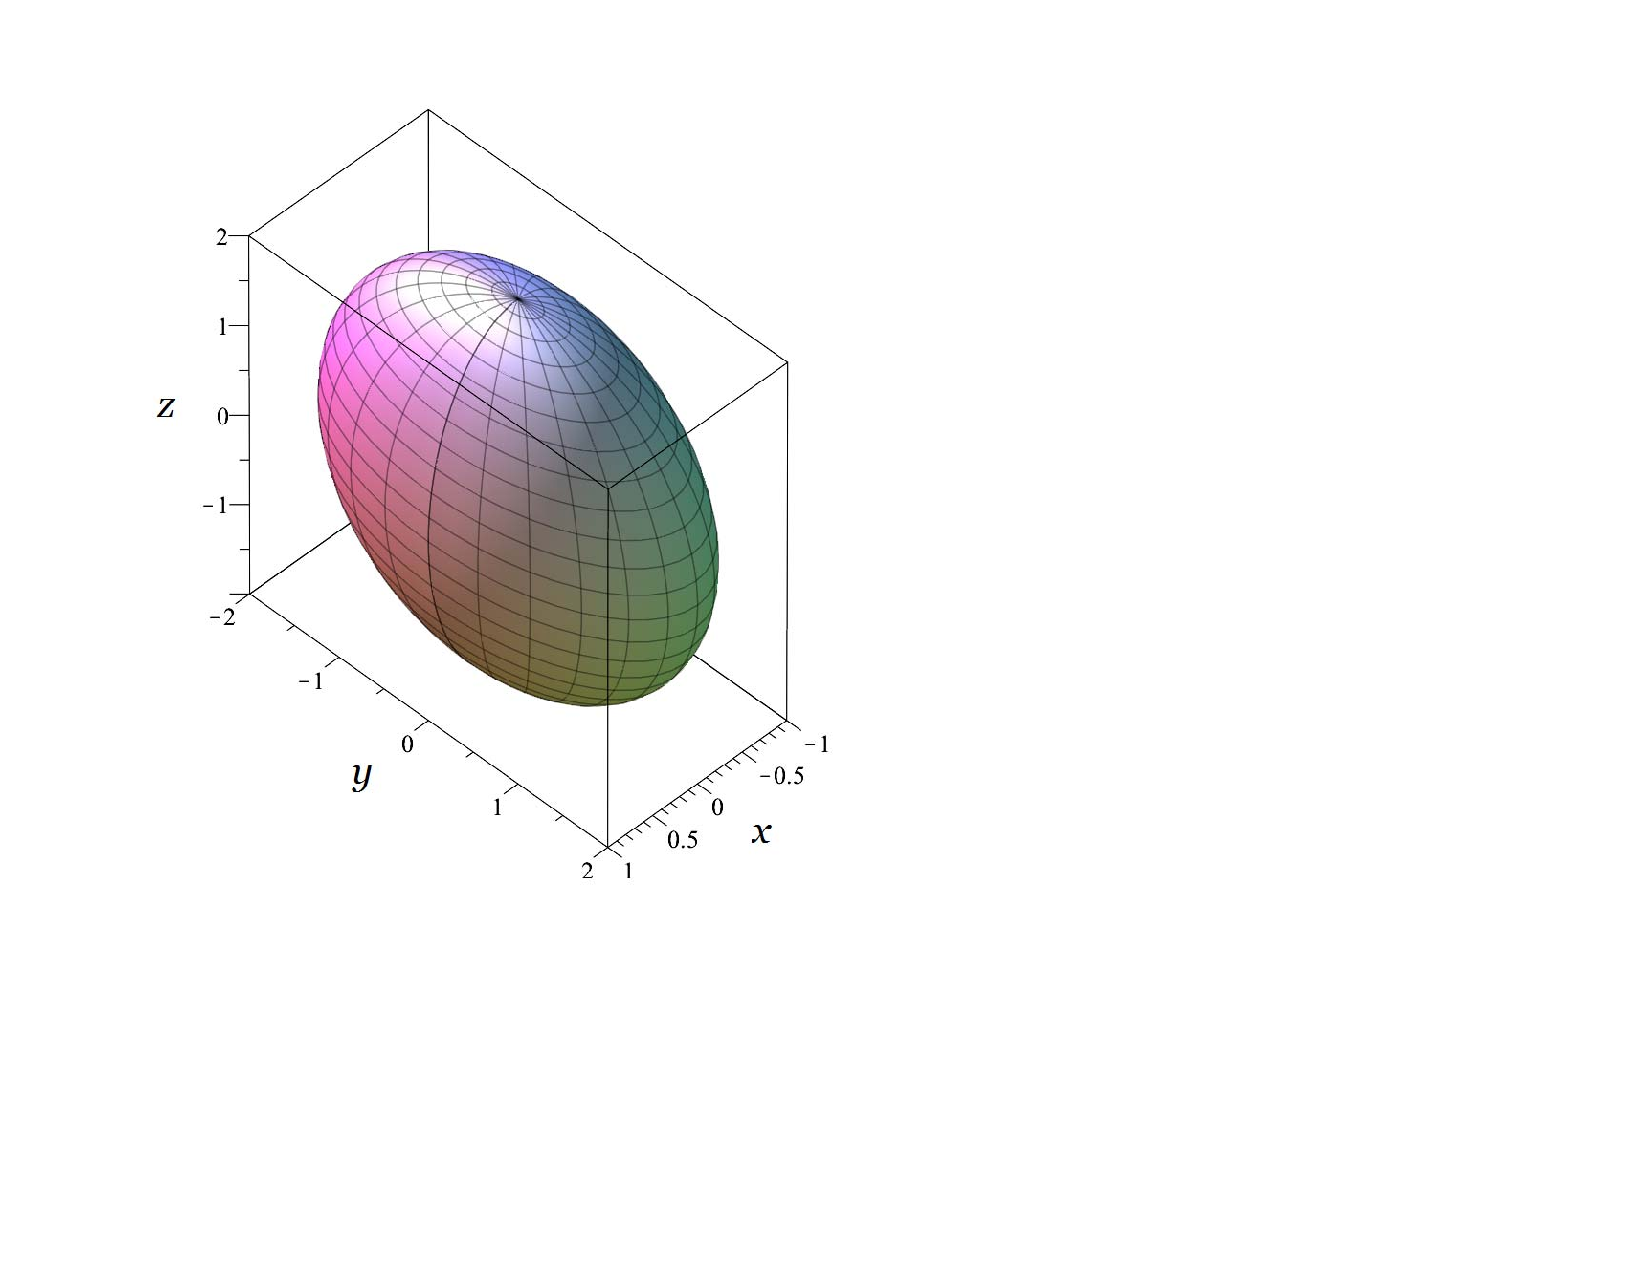
\includegraphics[scale=0.5]{ellipsoid.pdf}\end{center}}}} \fi

\newpage

\item $-x^2-y^2+z^2=1$

\ifans{\fbox{\parbox{0.45\linewidth}{\begin{center}Hyperboloid of 2 Sheets\\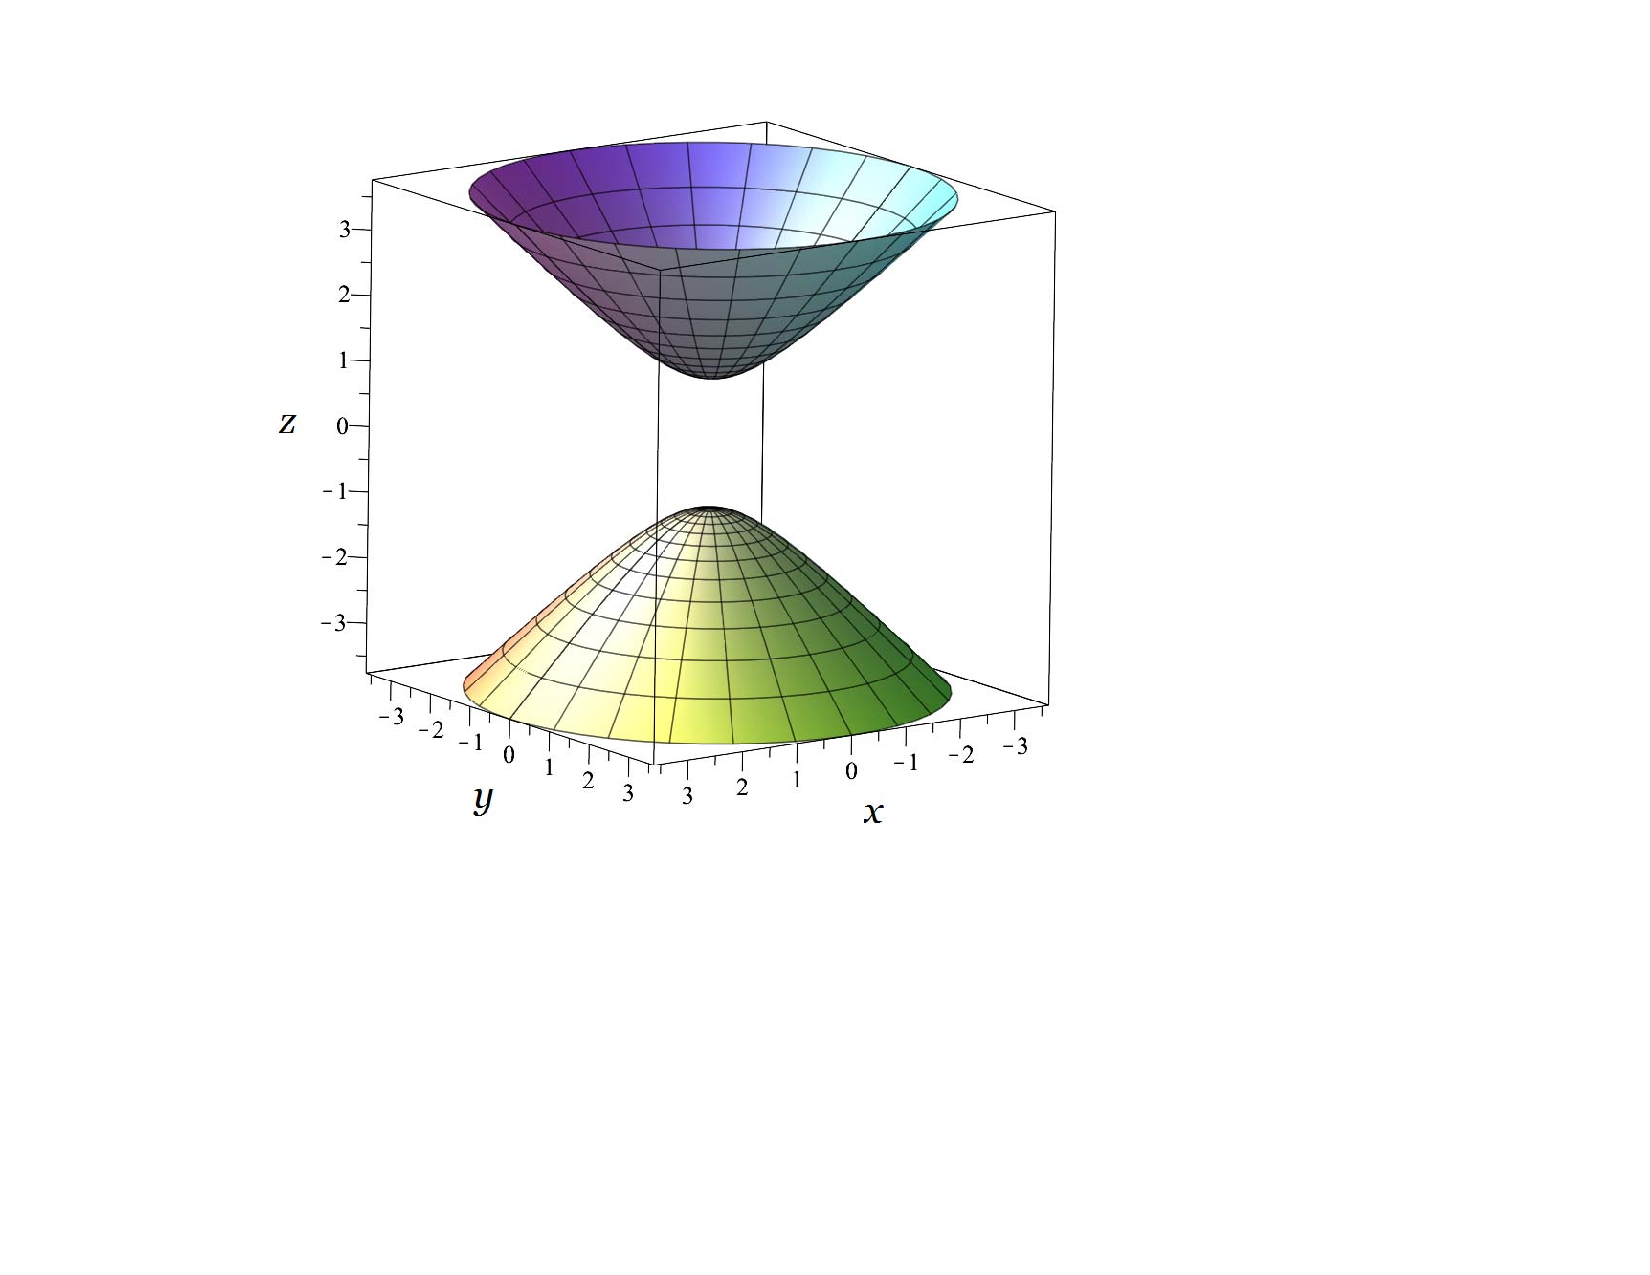
\includegraphics[scale=0.4]{hyperboloid2.pdf}\end{center}}}} \fi

\item $4x^2+9y^2-36z^2=36$

\ifans{\fbox{\parbox{0.45\linewidth}{\begin{center}Hyperboloid of 1 Sheet\\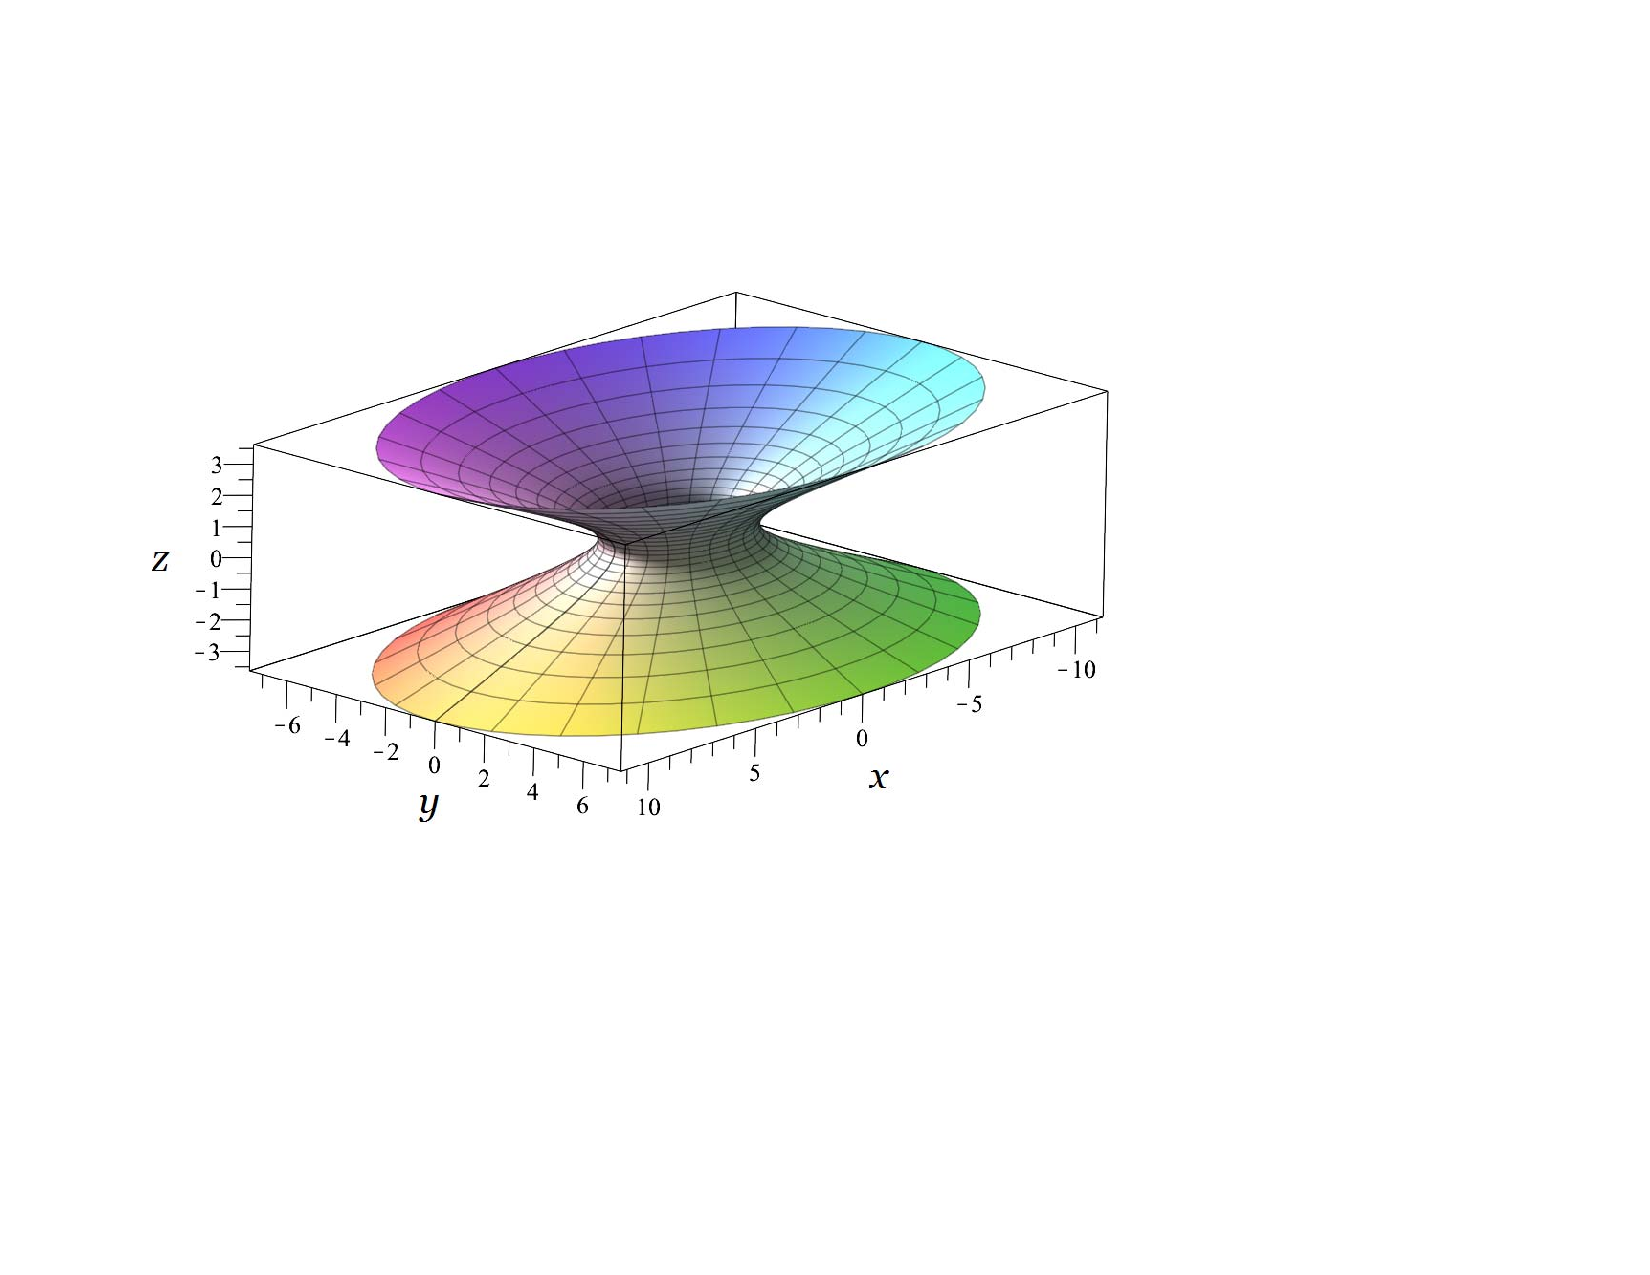
\includegraphics[scale=0.4]{hyperboloid1.pdf}\end{center}}}} \fi

\item $z=4x^2+y^2$

\ifans{\fbox{\parbox{0.45\linewidth}{\begin{center}Elliptic Paraboloid\\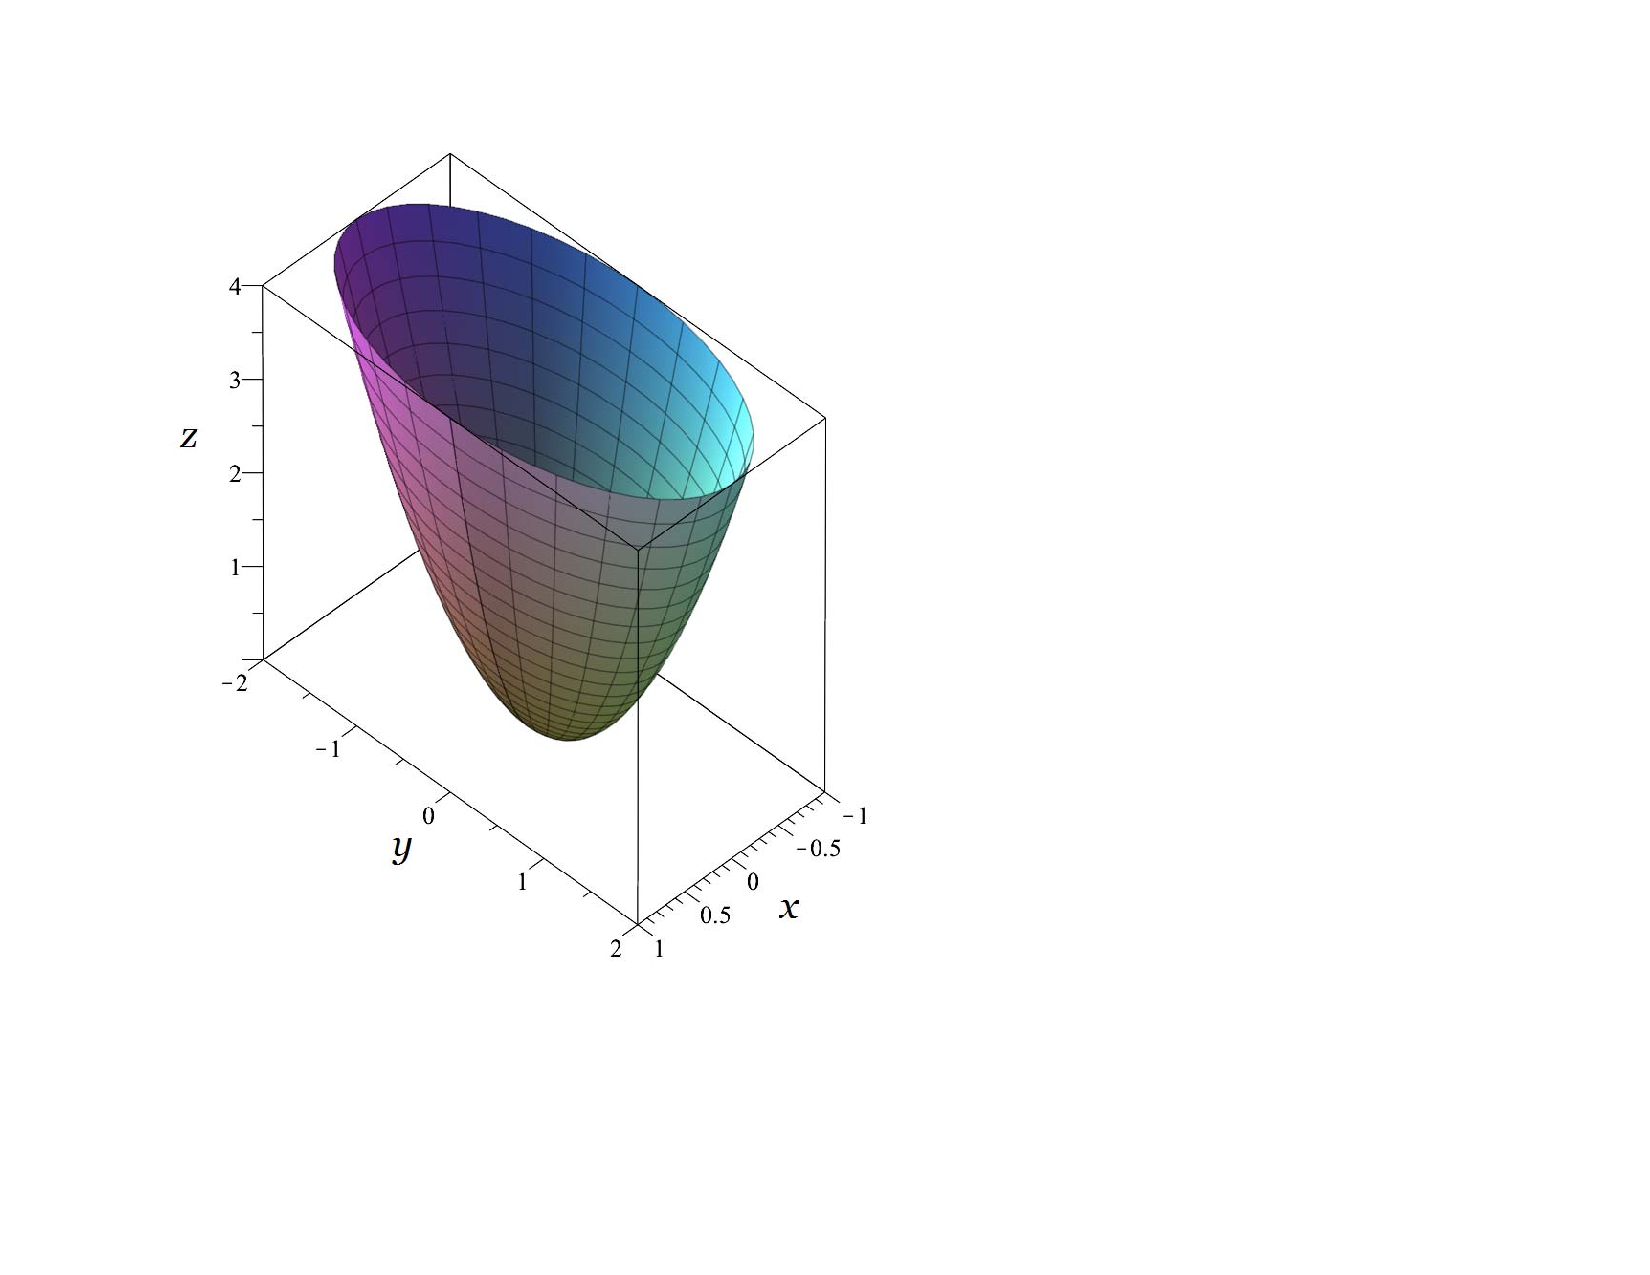
\includegraphics[scale=0.4]{paraboloid3.pdf}\end{center}}}} \fi

\item $z^2=x^2+y^2$

\ifans{\fbox{\parbox{0.45\linewidth}{\begin{center}Circular Double Cone\\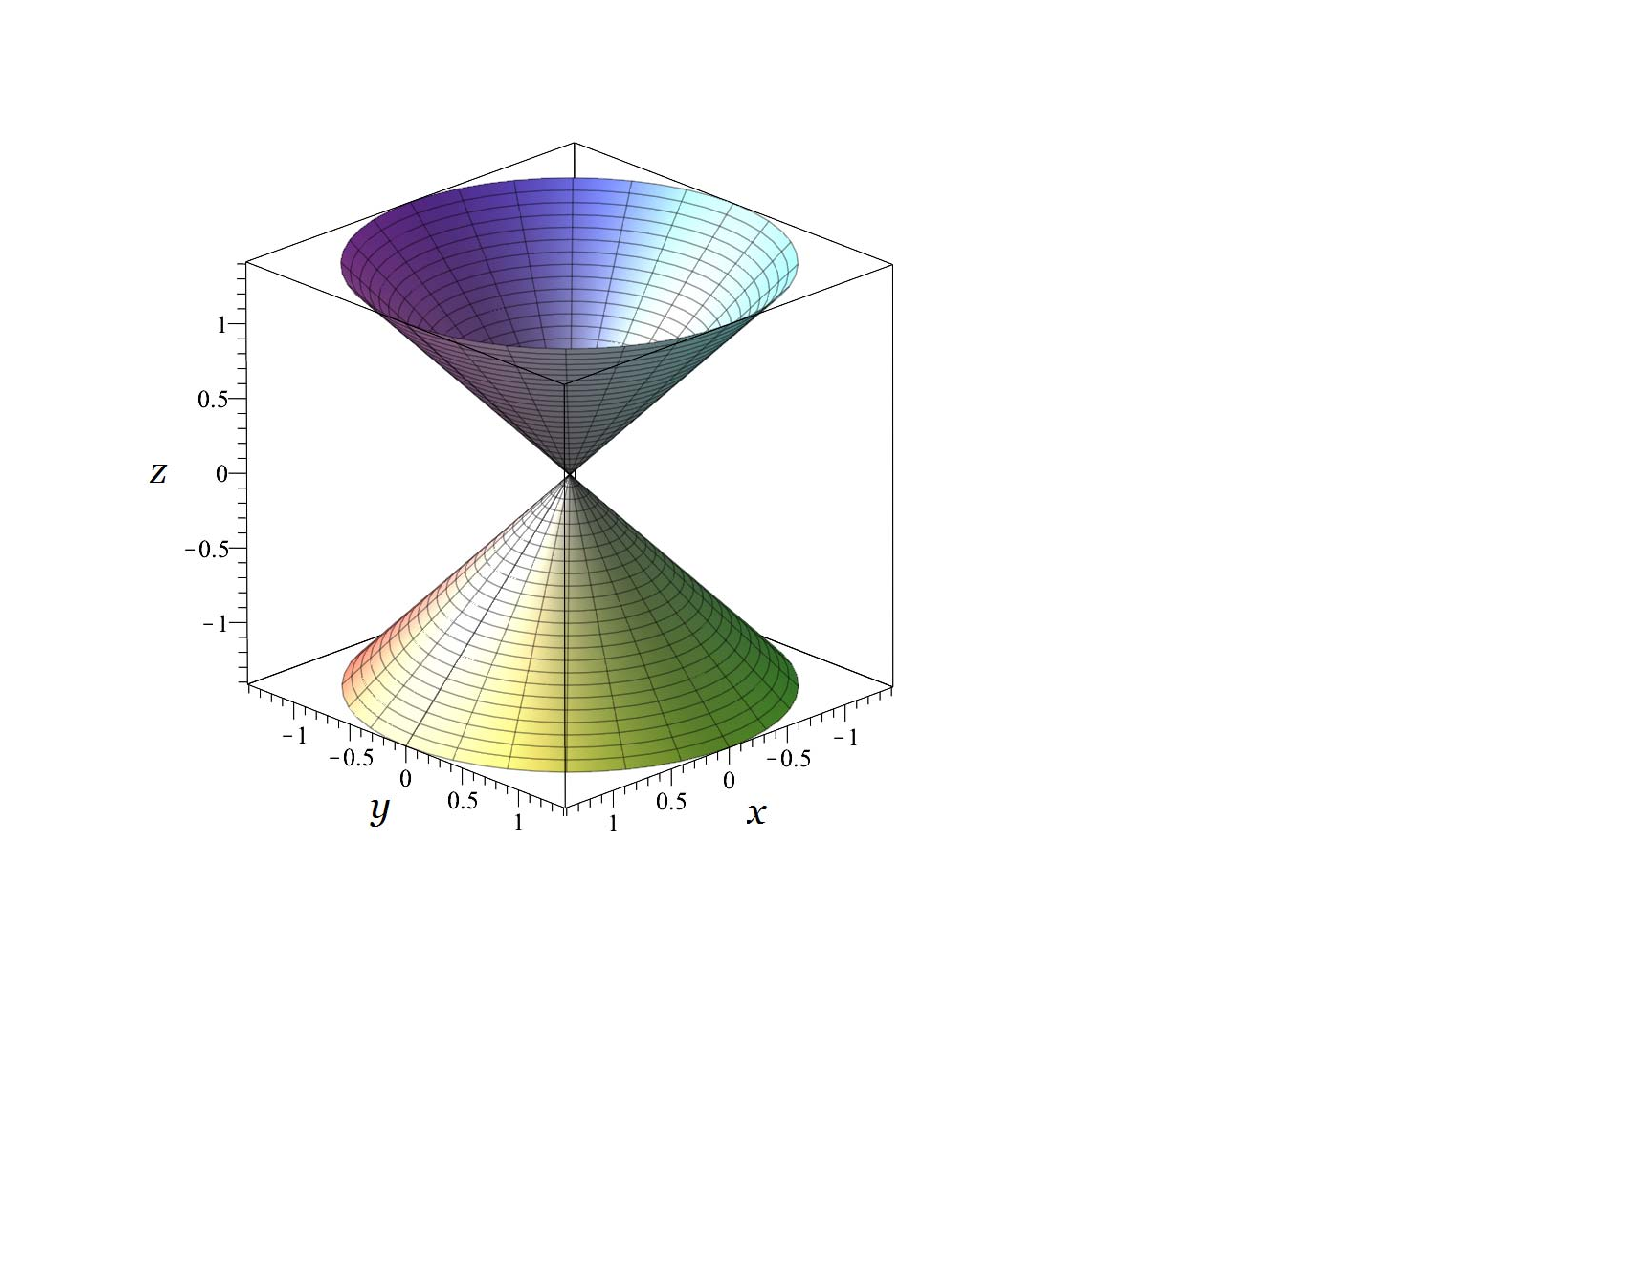
\includegraphics[scale=0.4]{cone1.pdf}\end{center}}}} \fi

\item $x^2+y^2-z^2=1$

\ifans{\fbox{\parbox{0.45\linewidth}{\begin{center}Hyperboloid of 1 Sheet\\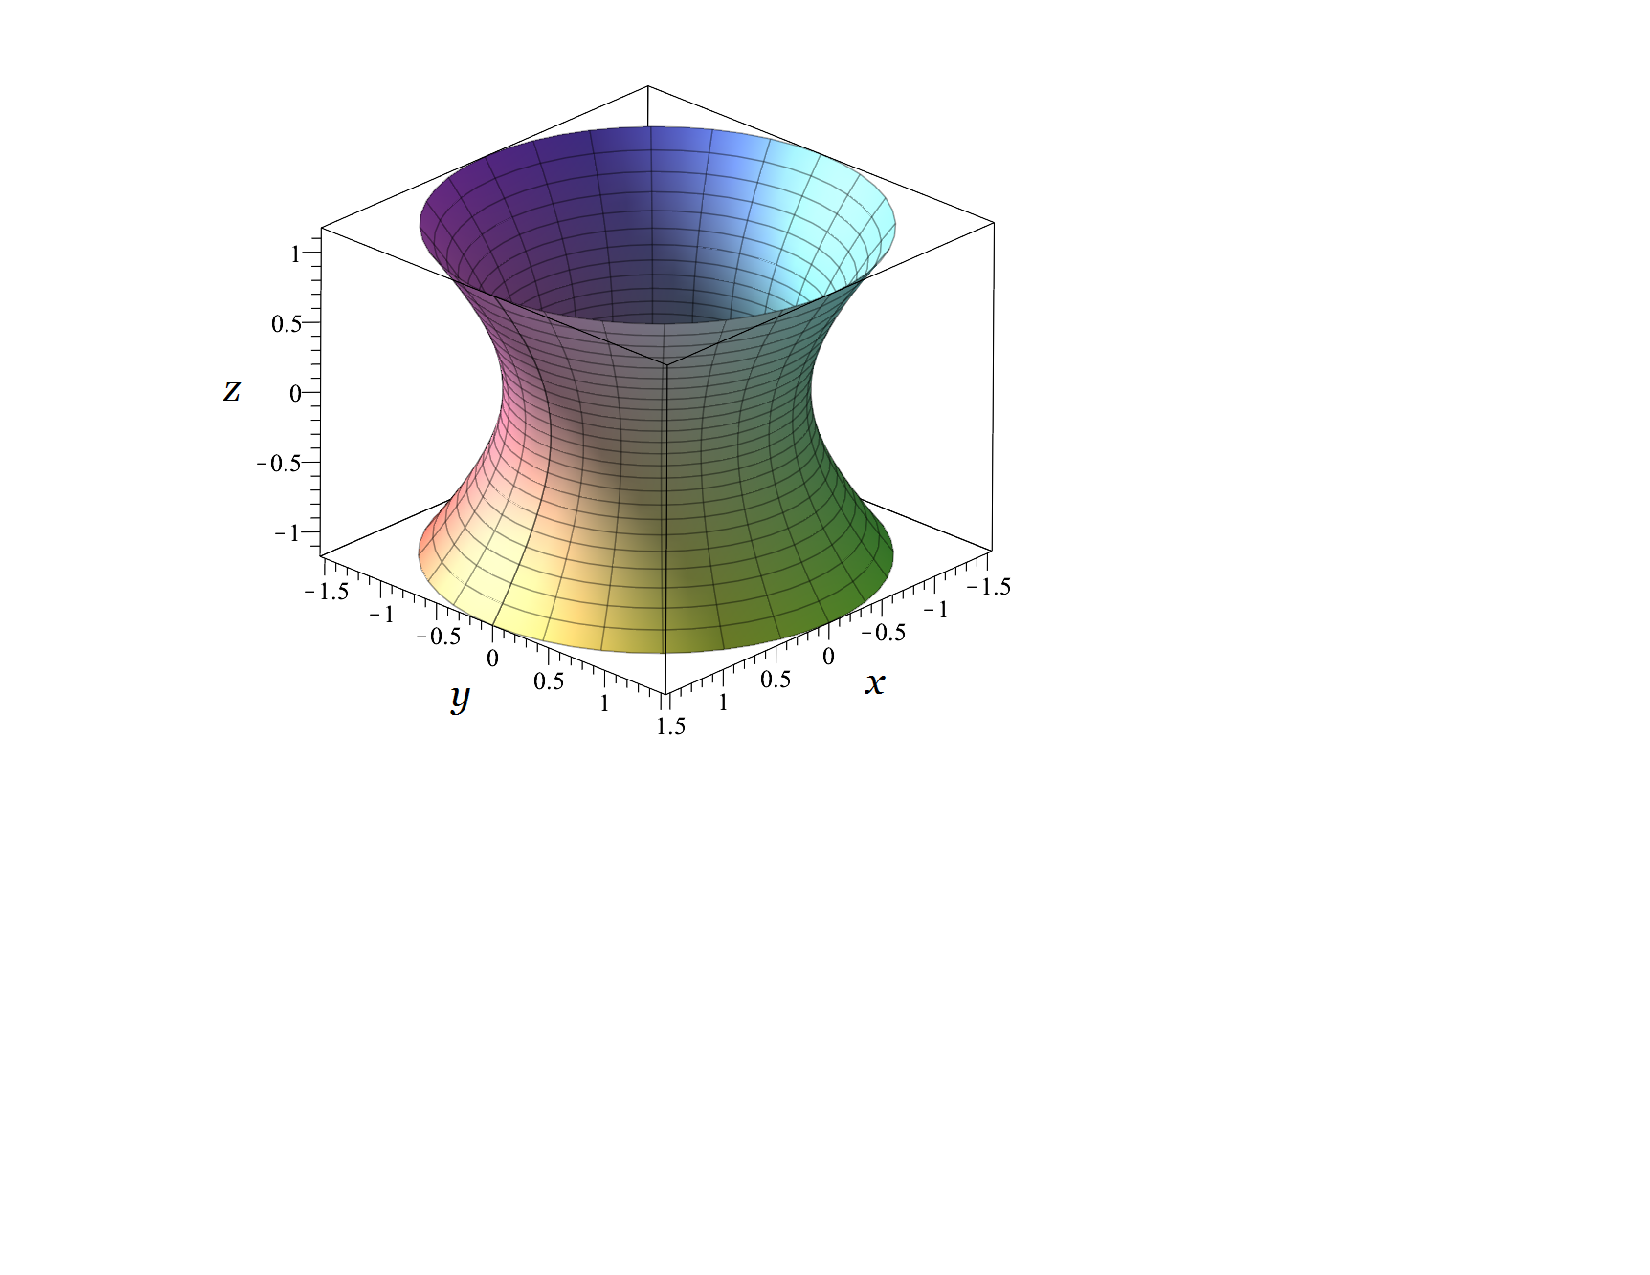
\includegraphics[scale=0.4]{hyperboloid.pdf}\end{center}}}} \fi

\item $z=4-x^2-y^2$

\ifans{\fbox{\parbox{0.45\linewidth}{\begin{center}Circular Paraboloid\\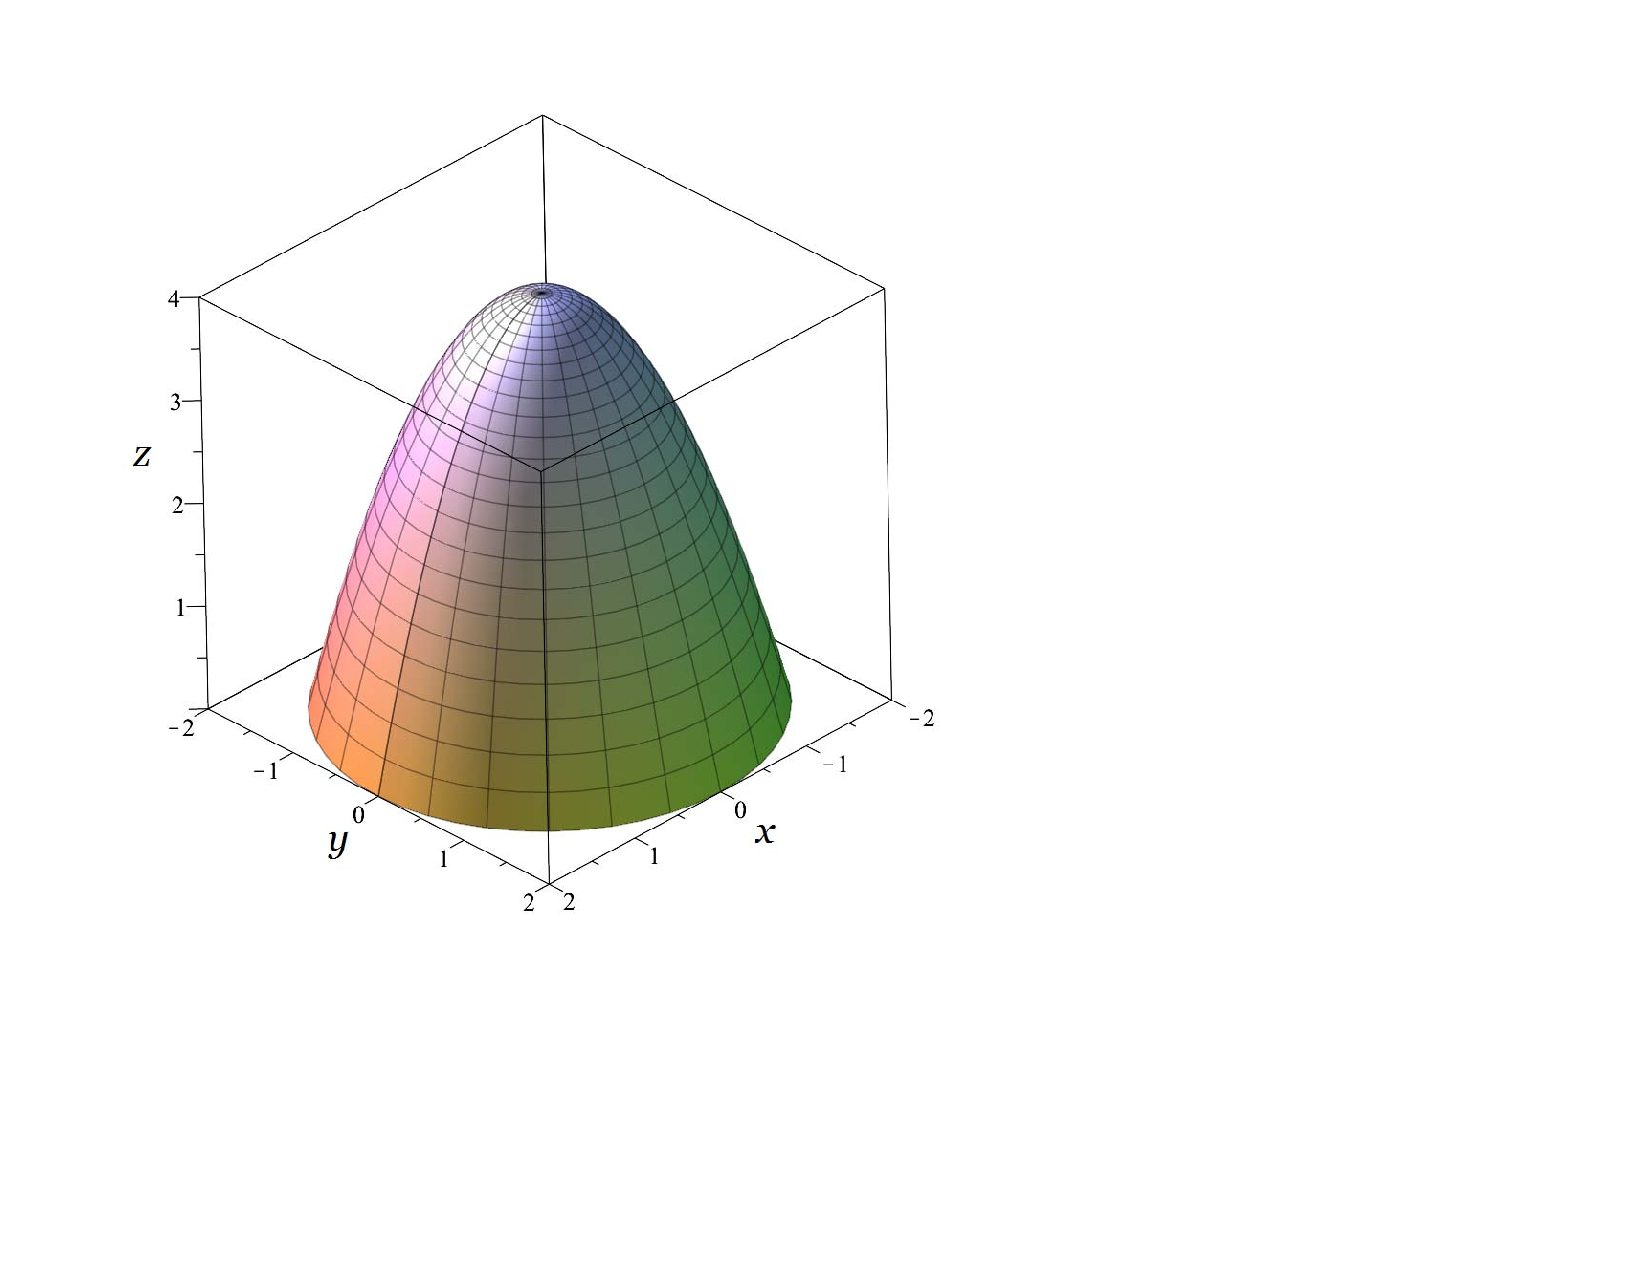
\includegraphics[scale=0.35]{paraboloid4.pdf}\end{center}}}} \fi

\item $3x^2+4y^2+6z^2=12$

\ifans{\fbox{\parbox{0.45\linewidth}{\begin{center}Ellipsoid\\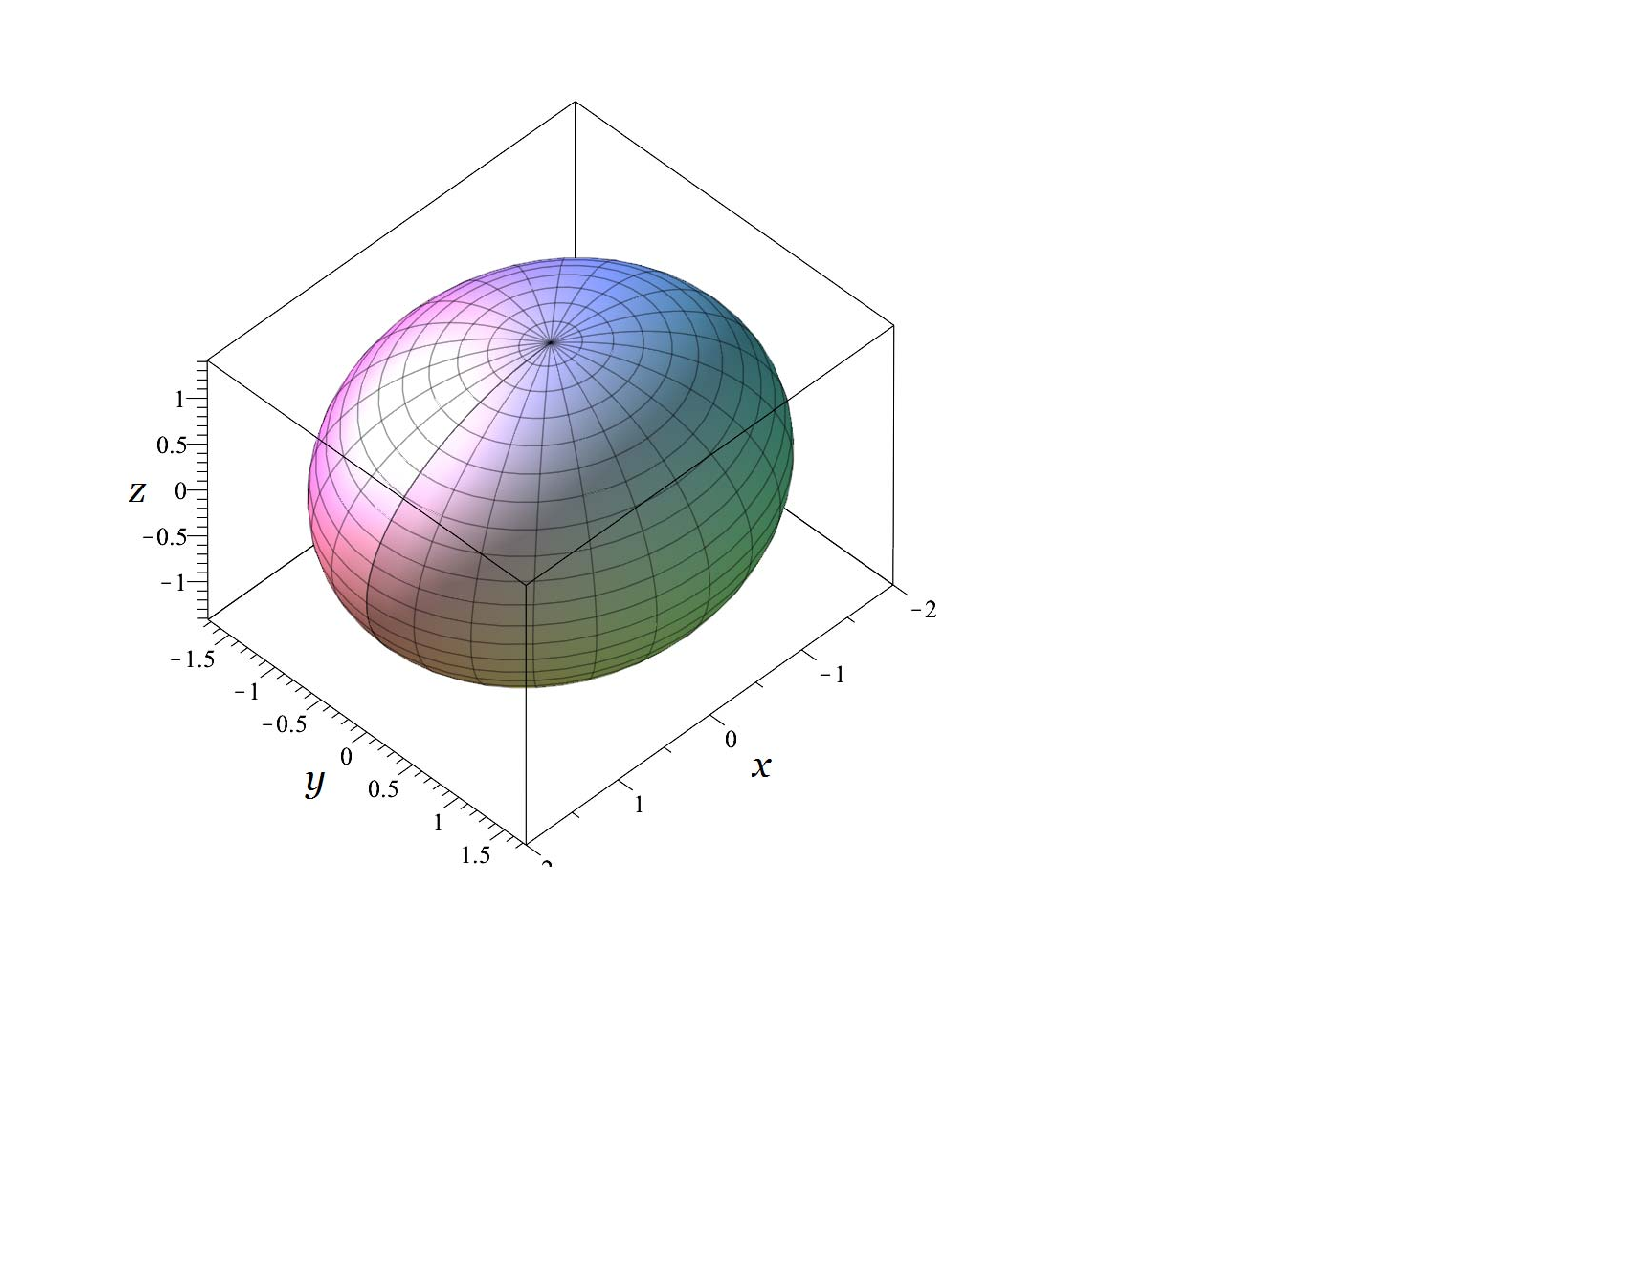
\includegraphics[scale=0.4]{ellipsoid2.pdf}\end{center}}}} \fi

\item $-4x^2-9y^2+36z^2=36$

\ifans{\fbox{\parbox{0.45\linewidth}{\begin{center}Hyperboloid of 2 Sheets\\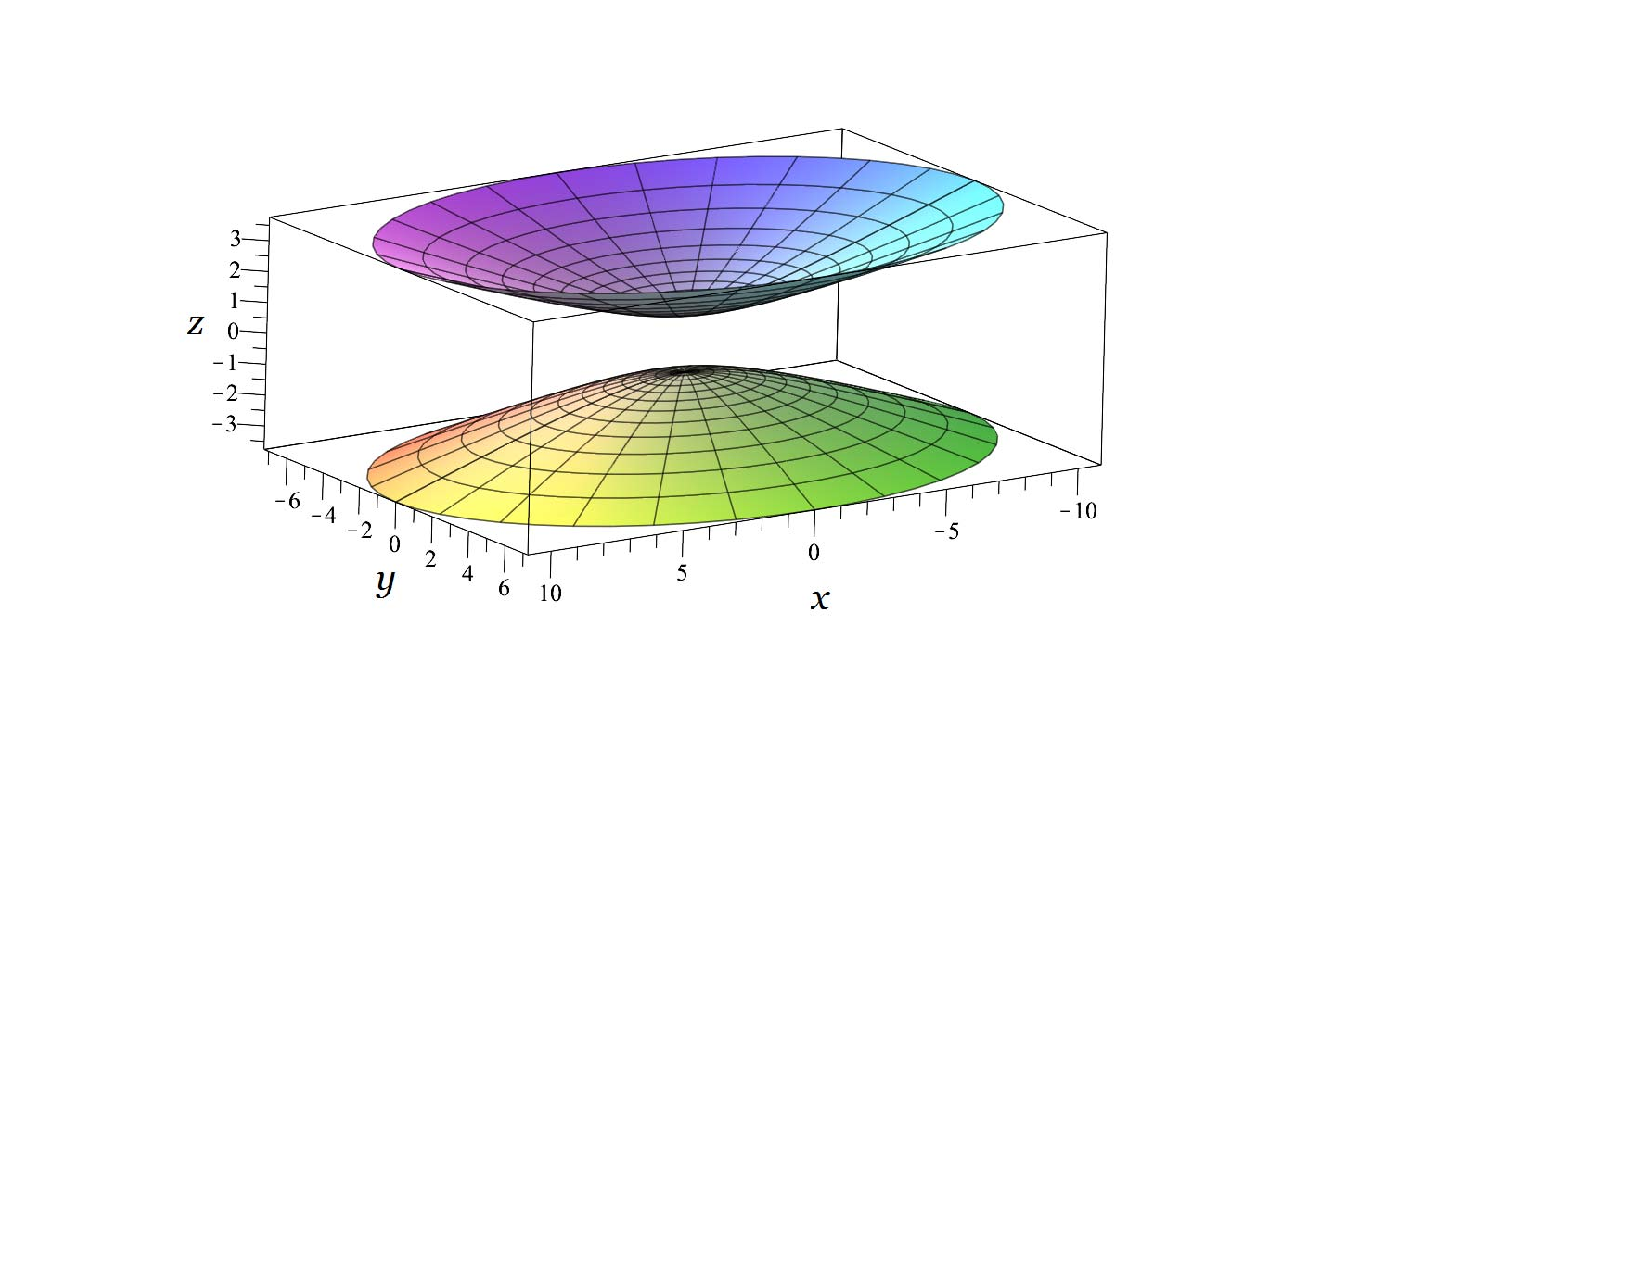
\includegraphics[scale=0.4]{hyperboloid3.pdf}\end{center}}}} \fi

\item Identify each of the following surfaces.

\begin{enumerate}

\item  $16x^2+4y^2+4z^2-64x+8y+16z=0$

\ifans{\fbox{\parbox{1\linewidth}{After completing the square, we can rewrite the equation as: $$16(x-2)^2+4(y+1)^2+4(z+2)^2=84$$
This is an ellipsoid which has been shifted.  Specifically, it is now centered at $(2,-1,-2)$.
}}} \fi

\item $-4x^2+y^2+16z^2-8x+10y+32z=0$

\ifans{\fbox{\parbox{1\linewidth}{After completing the square, we can rewrite the equation as: $$-4(x-1)^2+(y+5)^2+16(z+1)^2=37$$
This is a hyperboloid of 1 sheet which has been shifted.  Specifically, its central axis is parallel to the $x$-axis.  In fact, the equation of its central axis is $\overrightarrow{\ell}(t)=\langle 1,-5,-1 \rangle +t \langle 1, 0, 0 \rangle$.
}}} \fi

\end{enumerate}

\item Consider the paraboloid $z=x^2+y^2$

\begin{enumerate}

\item Compute equations for the traces in the $z=0$, $z=1$, $z=2$, and $z=3$ planes.

\ifans{\fbox{\parbox{0.4\linewidth}{\begin{center}
\begin{tabular}{l|c}
{\bf Plane} & {\bf Trace}\\
\hline
$z=0$ & Point $(0,0)$\\
$z=1$ & Circle $x^2+y^2=1$\\
$z=2$ & Circle $x^2+y^2=2$\\
$z=3$ & Circle $x^2+y^2=3$\\
\end{tabular}
\end{center}
}}} \fi

\item Sketch all the traces that you found in part (a) on the same coordinate axes.

\ifans{\fbox{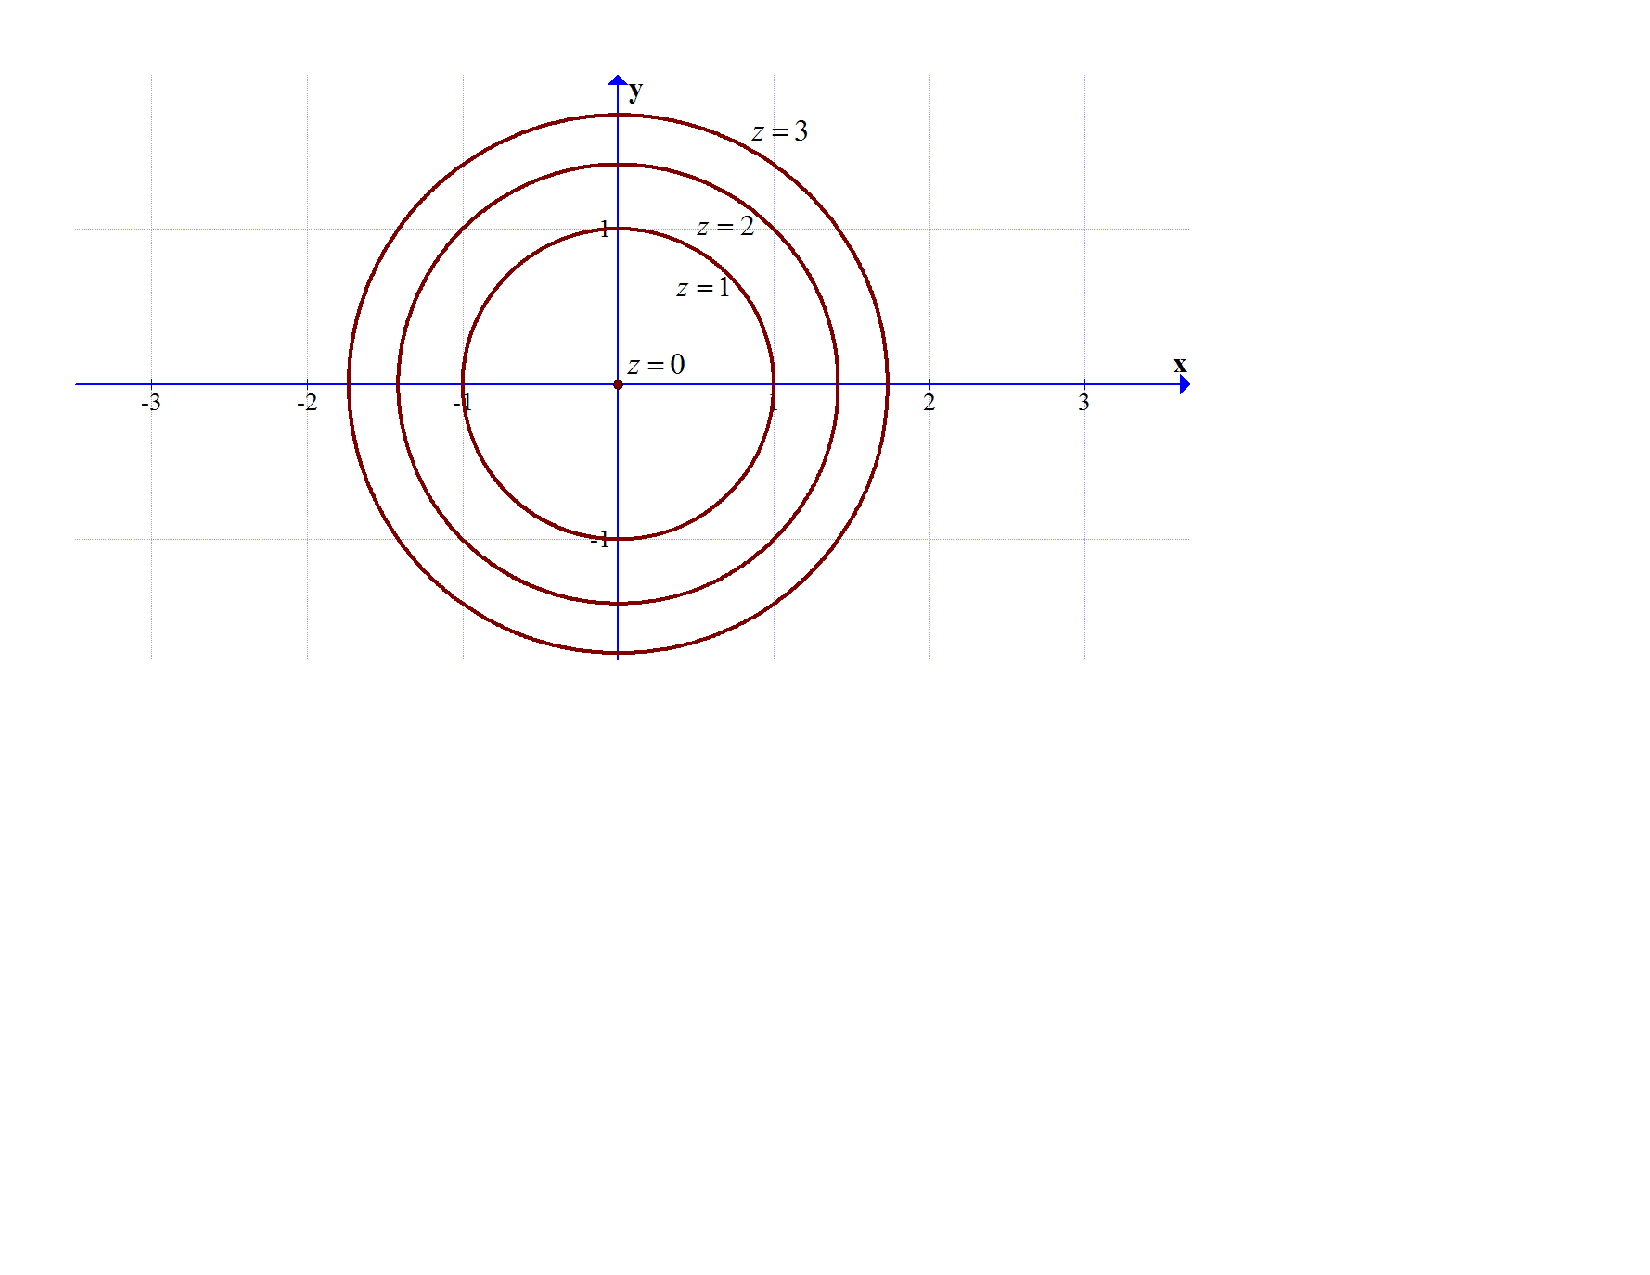
\includegraphics[scale=0.33]{traces.pdf}}} \fi

\item Compute equations for the traces in the $y=0$, $y=1$, $y=2$, and $y=3$ planes.

\ifans{\fbox{\parbox{0.4\linewidth}{\begin{center}
\begin{tabular}{l|c}
{\bf Plane} & {\bf Trace}\\
\hline
$y=0$ & Parabola $z=x^2$\\
$y=1$ & Parabola $z=x^2+1$\\
$y=2$ & Parabola $z=x^2+4$\\
$y=3$ & Parabola $z=x^2+9$\\
\end{tabular}
\end{center}
}}} \fi

\item Sketch all the traces that you found in part (c) on the same coordinate axes.

\ifans{\fbox{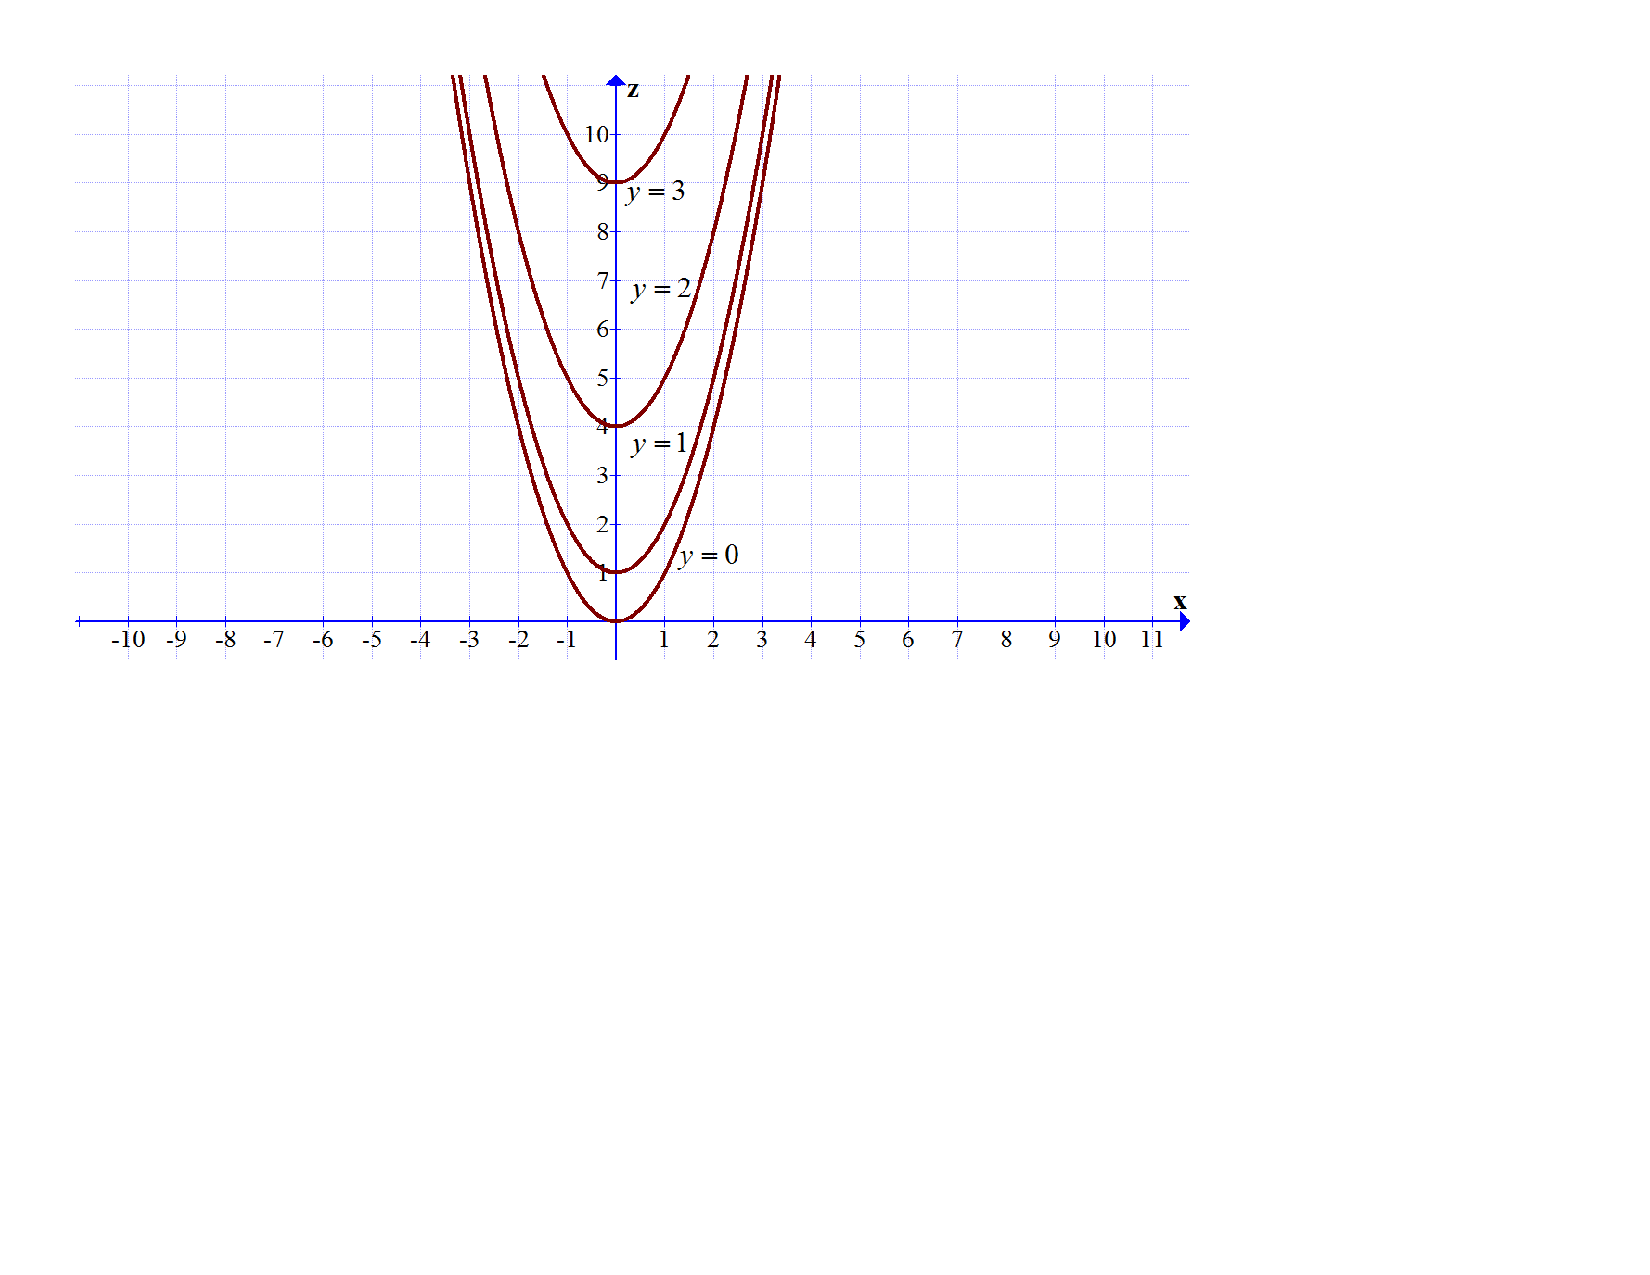
\includegraphics[scale=0.33]{traces2.pdf}}} \fi

\item Below is the graph of $z=x^2+y^2$.  On the graph of the surface, sketch the traces that you found in parts (a) and (c).

\begin{center}
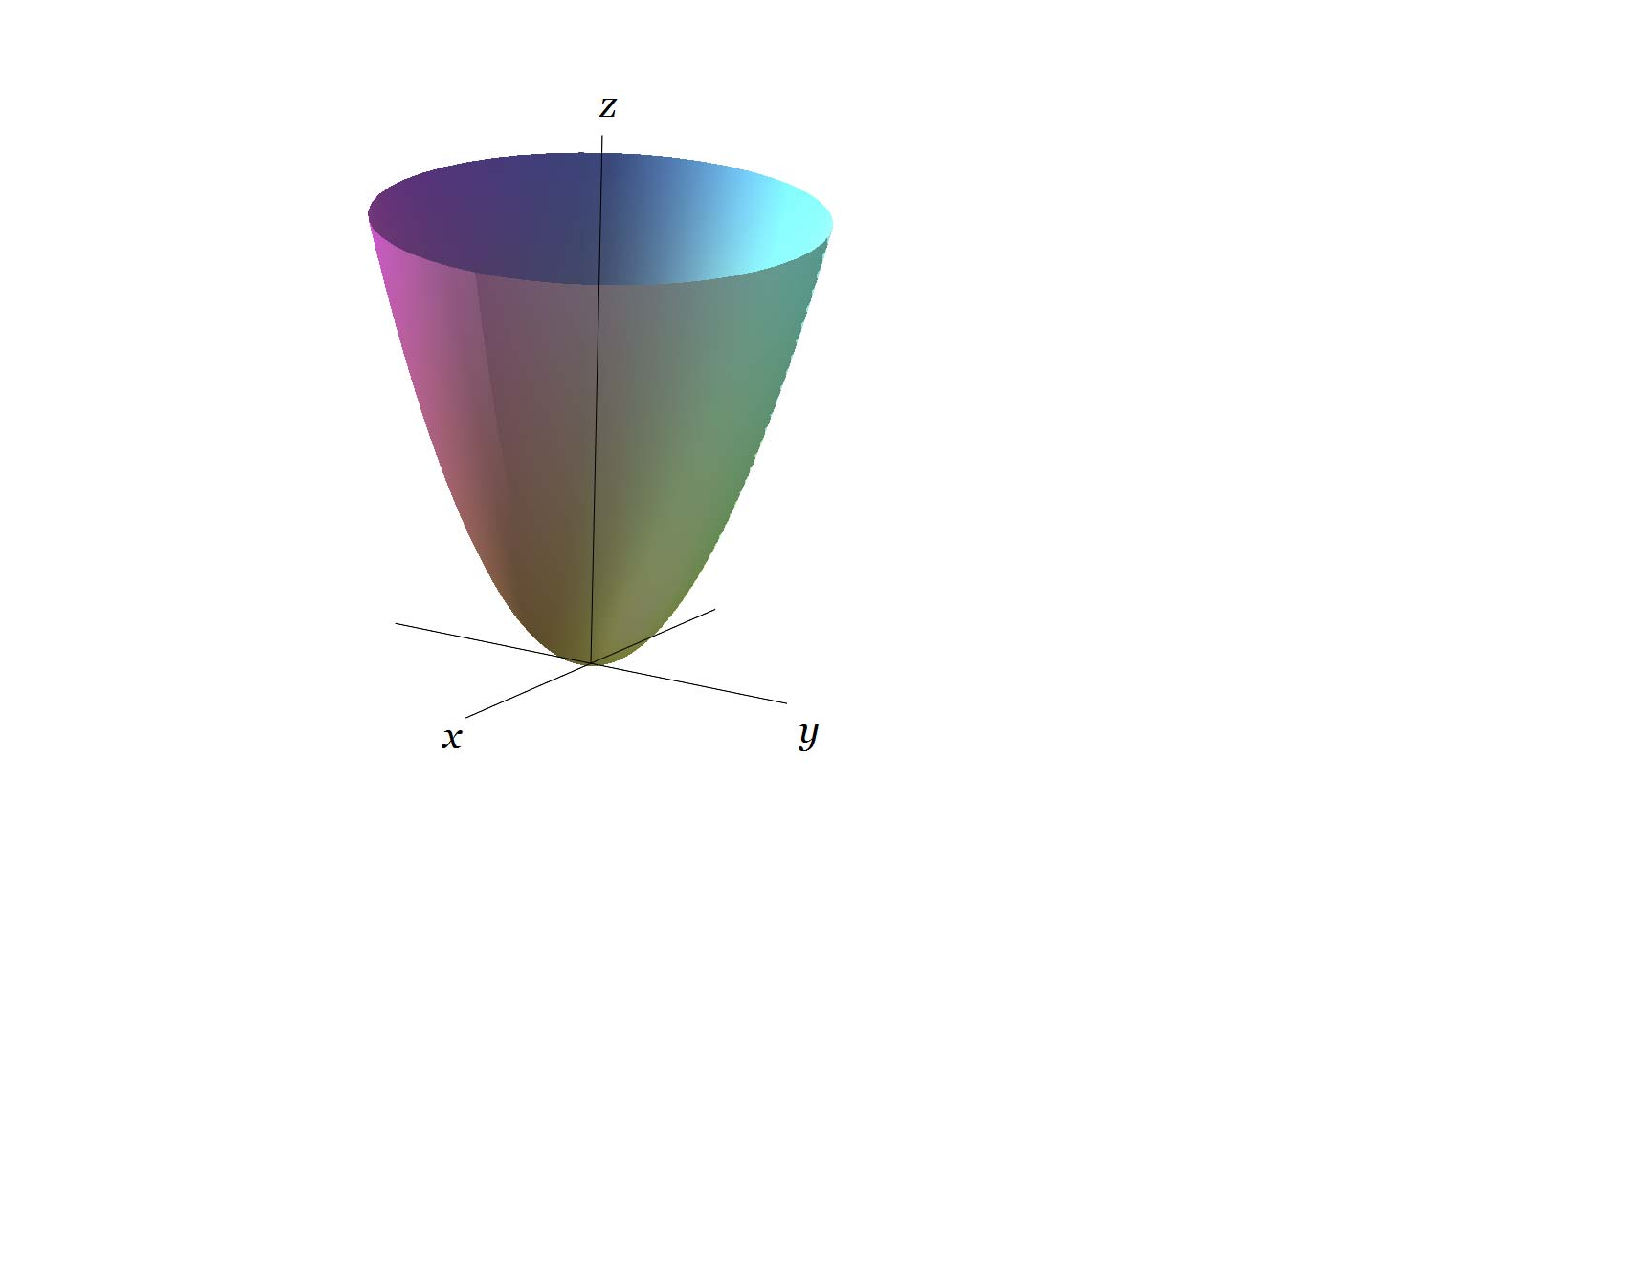
\includegraphics[scale=0.6]{paraboloid_trace.pdf}
\end{center}

\end{enumerate}

\end{enumerate}

\noindent {\bf For problems 12-13, find an equation of the trace of the surface in the indicated plane.  Describe the graph of the trace.}

\begin{enumerate}
\setcounter{enumi}{11}

\item Surface: $8x^2+y^2+z^2=9$; Plane: $z=1$

\ifans{\fbox{\parbox{1\linewidth}{\begin{center}The trace in the $z=1$ plane is the ellipse $x^2+\frac{y^2}{8}=1$, shown below.\\
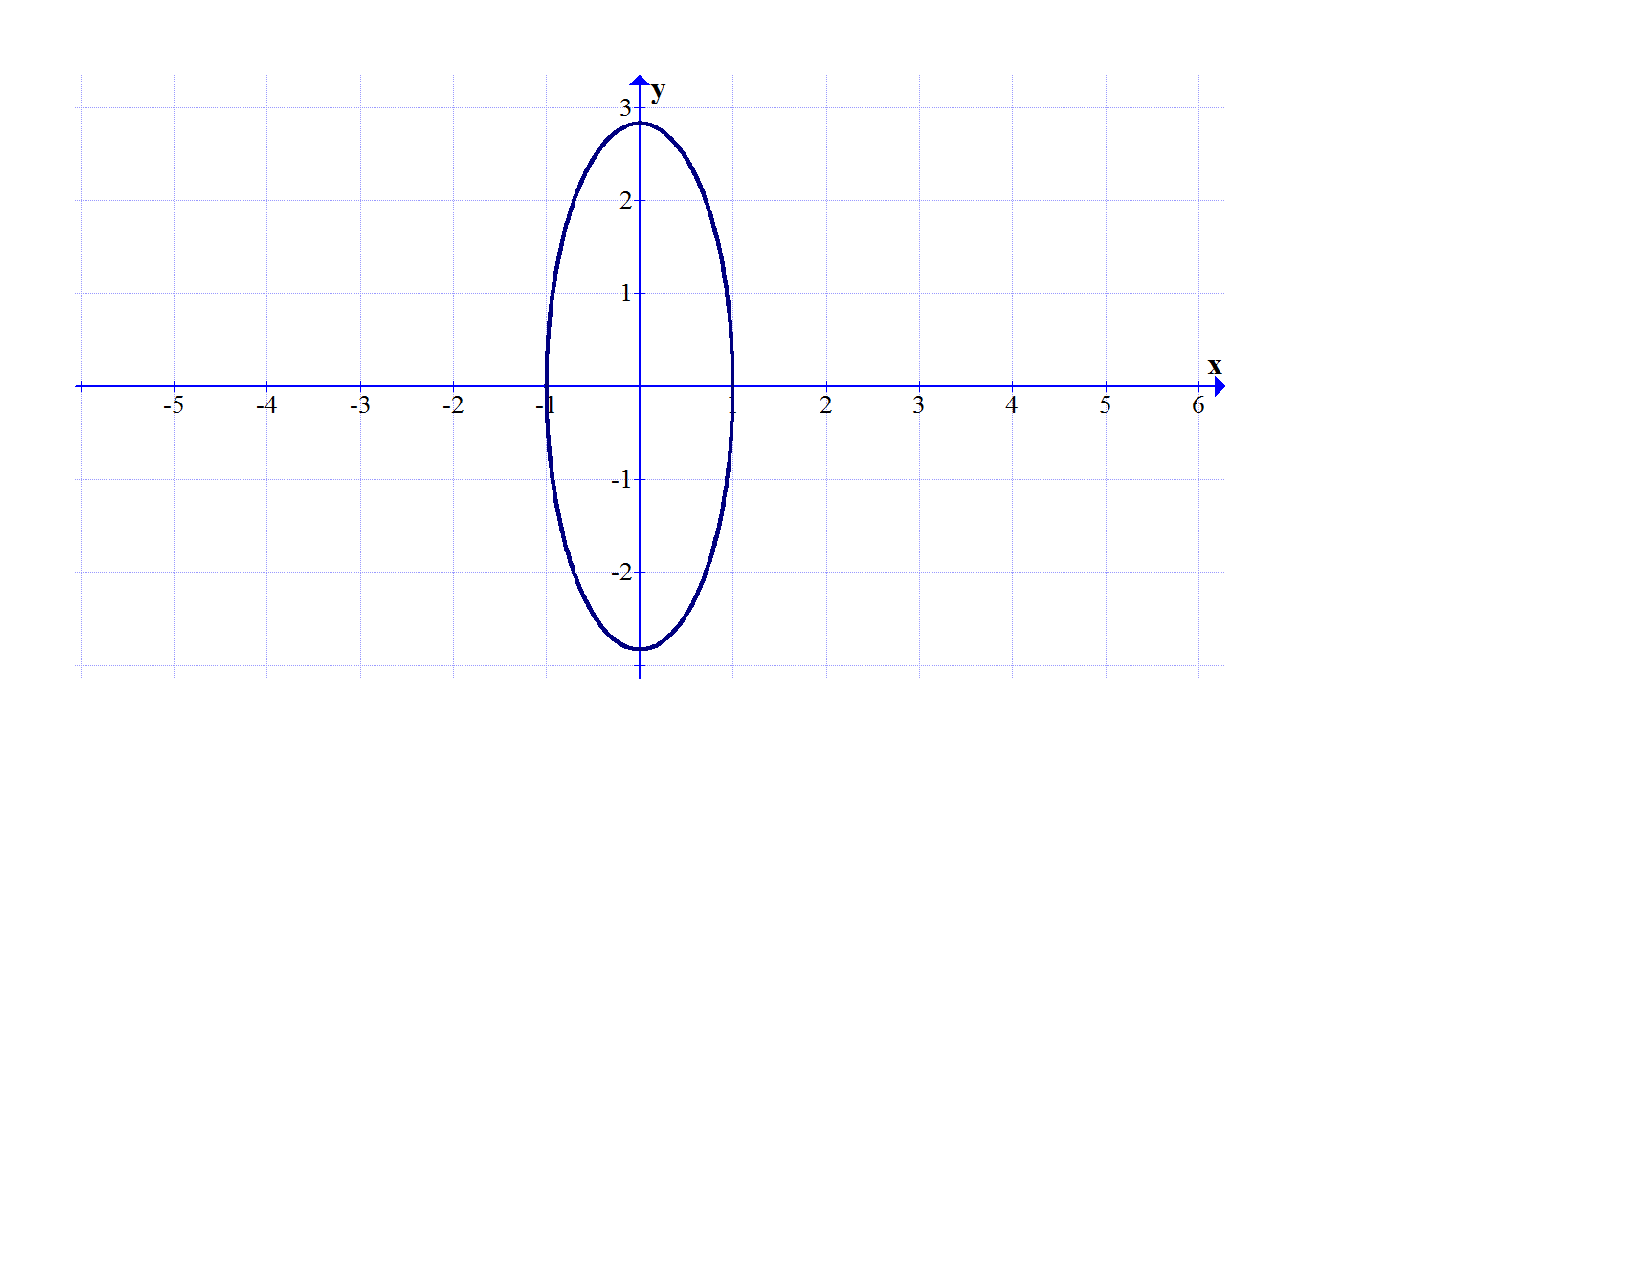
\includegraphics[scale=0.5]{trace1.pdf}
\end{center}}}} \fi

\newpage

\item Surface: $-4x^2-4y^2+9z^2=35$; Plane $x=\frac{1}{2}$

\ifans{\fbox{\parbox{1\linewidth}{\begin{center}The trace in the $x=\frac{1}{2}$ plane is the hyperbola $-\frac{y^2}{9}+\frac{z^2}{4}=1$, shown below.\\
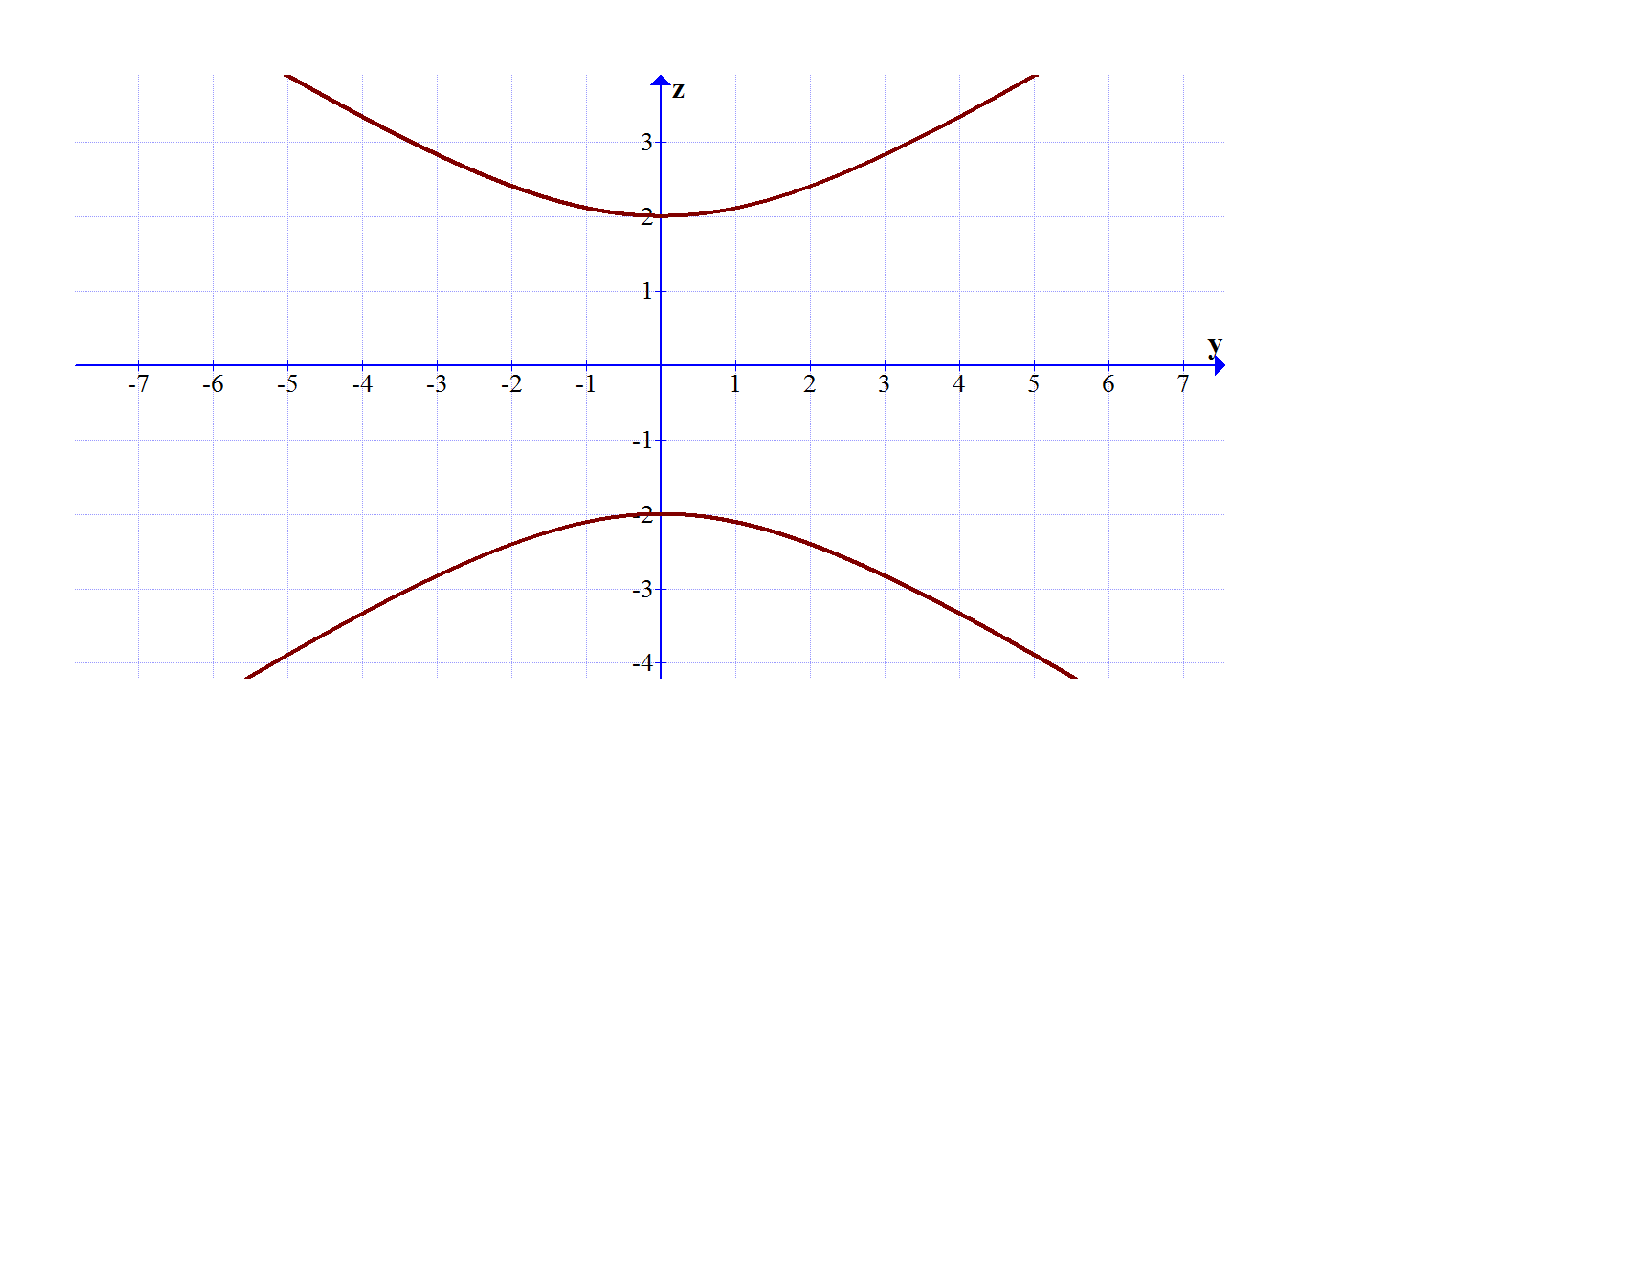
\includegraphics[scale=0.4]{traces3.pdf}
\end{center}}}} \fi

\end{enumerate}

\noindent {\bf For problems 14-15, sketch the indicated region.}

\begin{enumerate}
\setcounter{enumi}{13}

\item The region bounded below by $z=\sqrt{x^2+y^2}$ and bounded above by $z=2-x^2-y^2$.

\ifans{\fbox{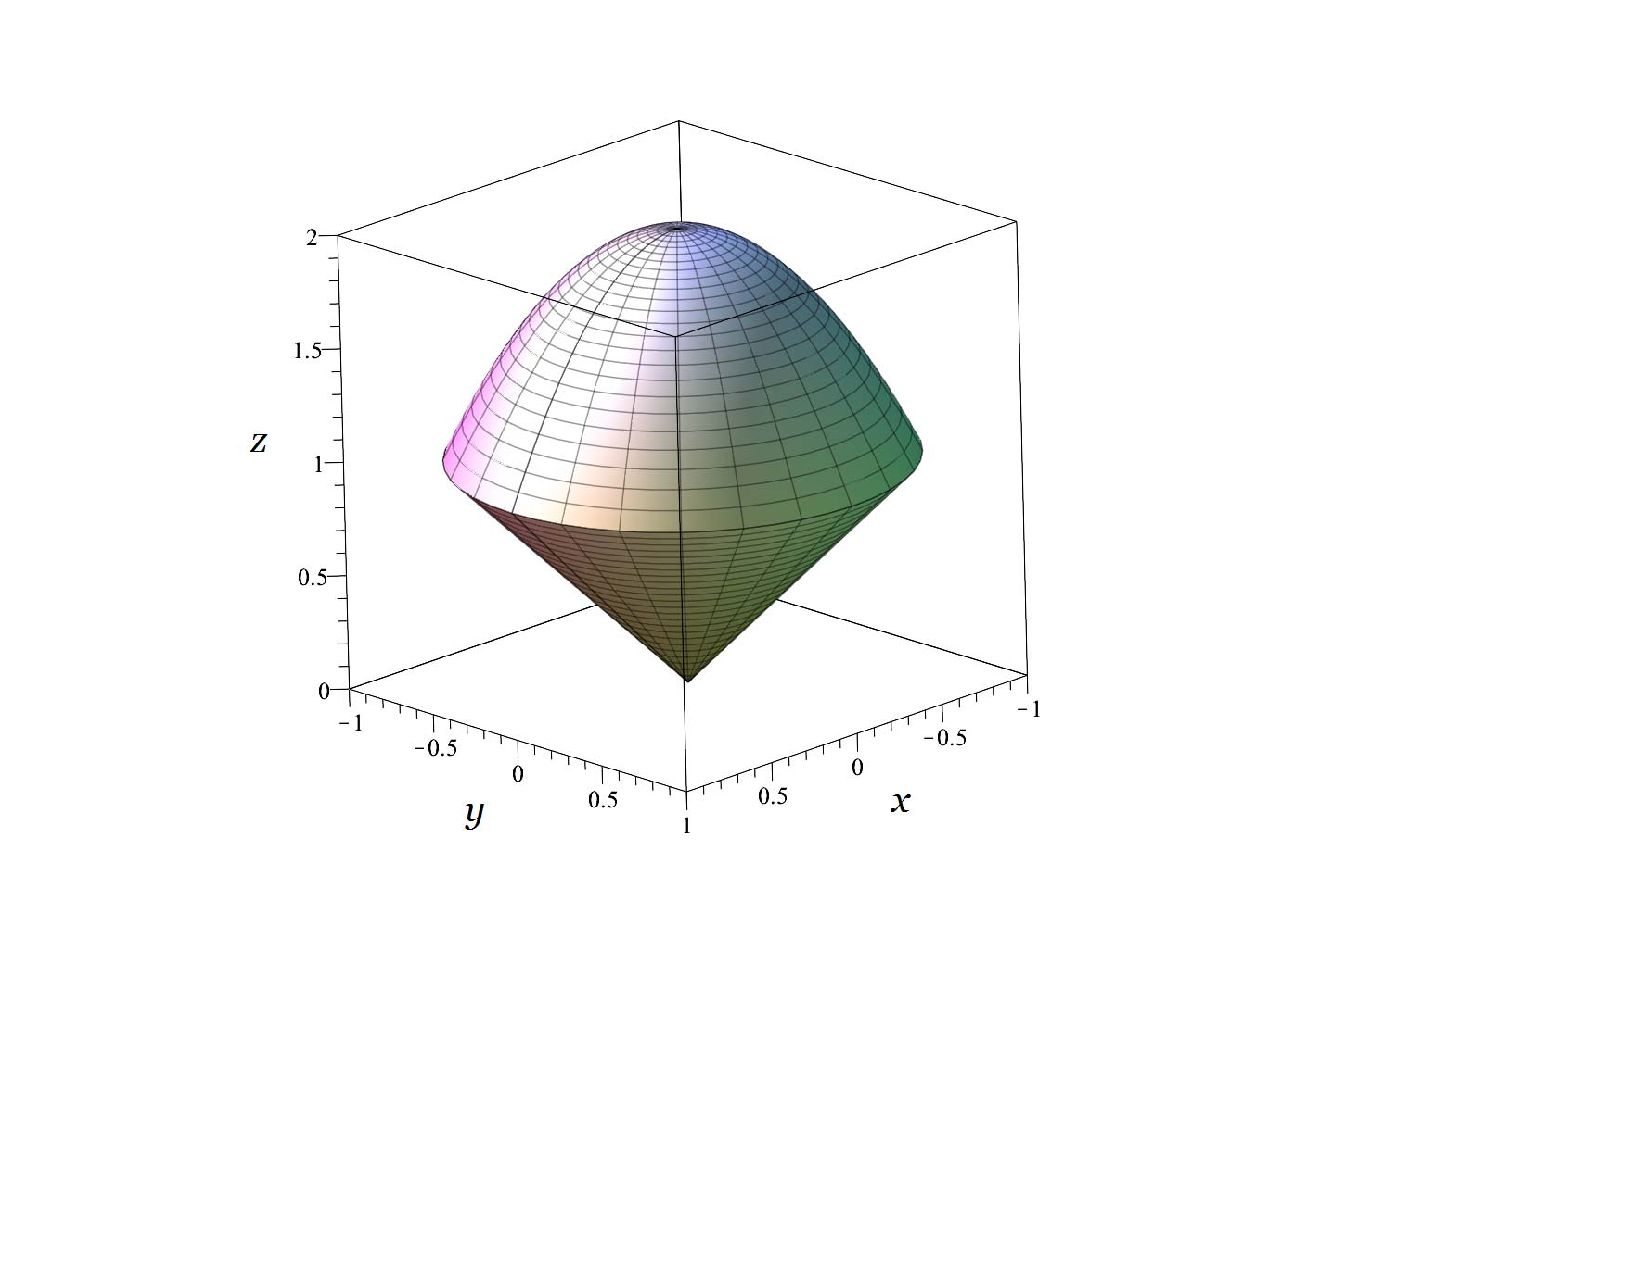
\includegraphics[scale=0.4]{top.pdf}}} \fi

\item The region bounded below by $2z=x^2+y^2$ and bounded above by $z=y$.

\ifans{\fbox{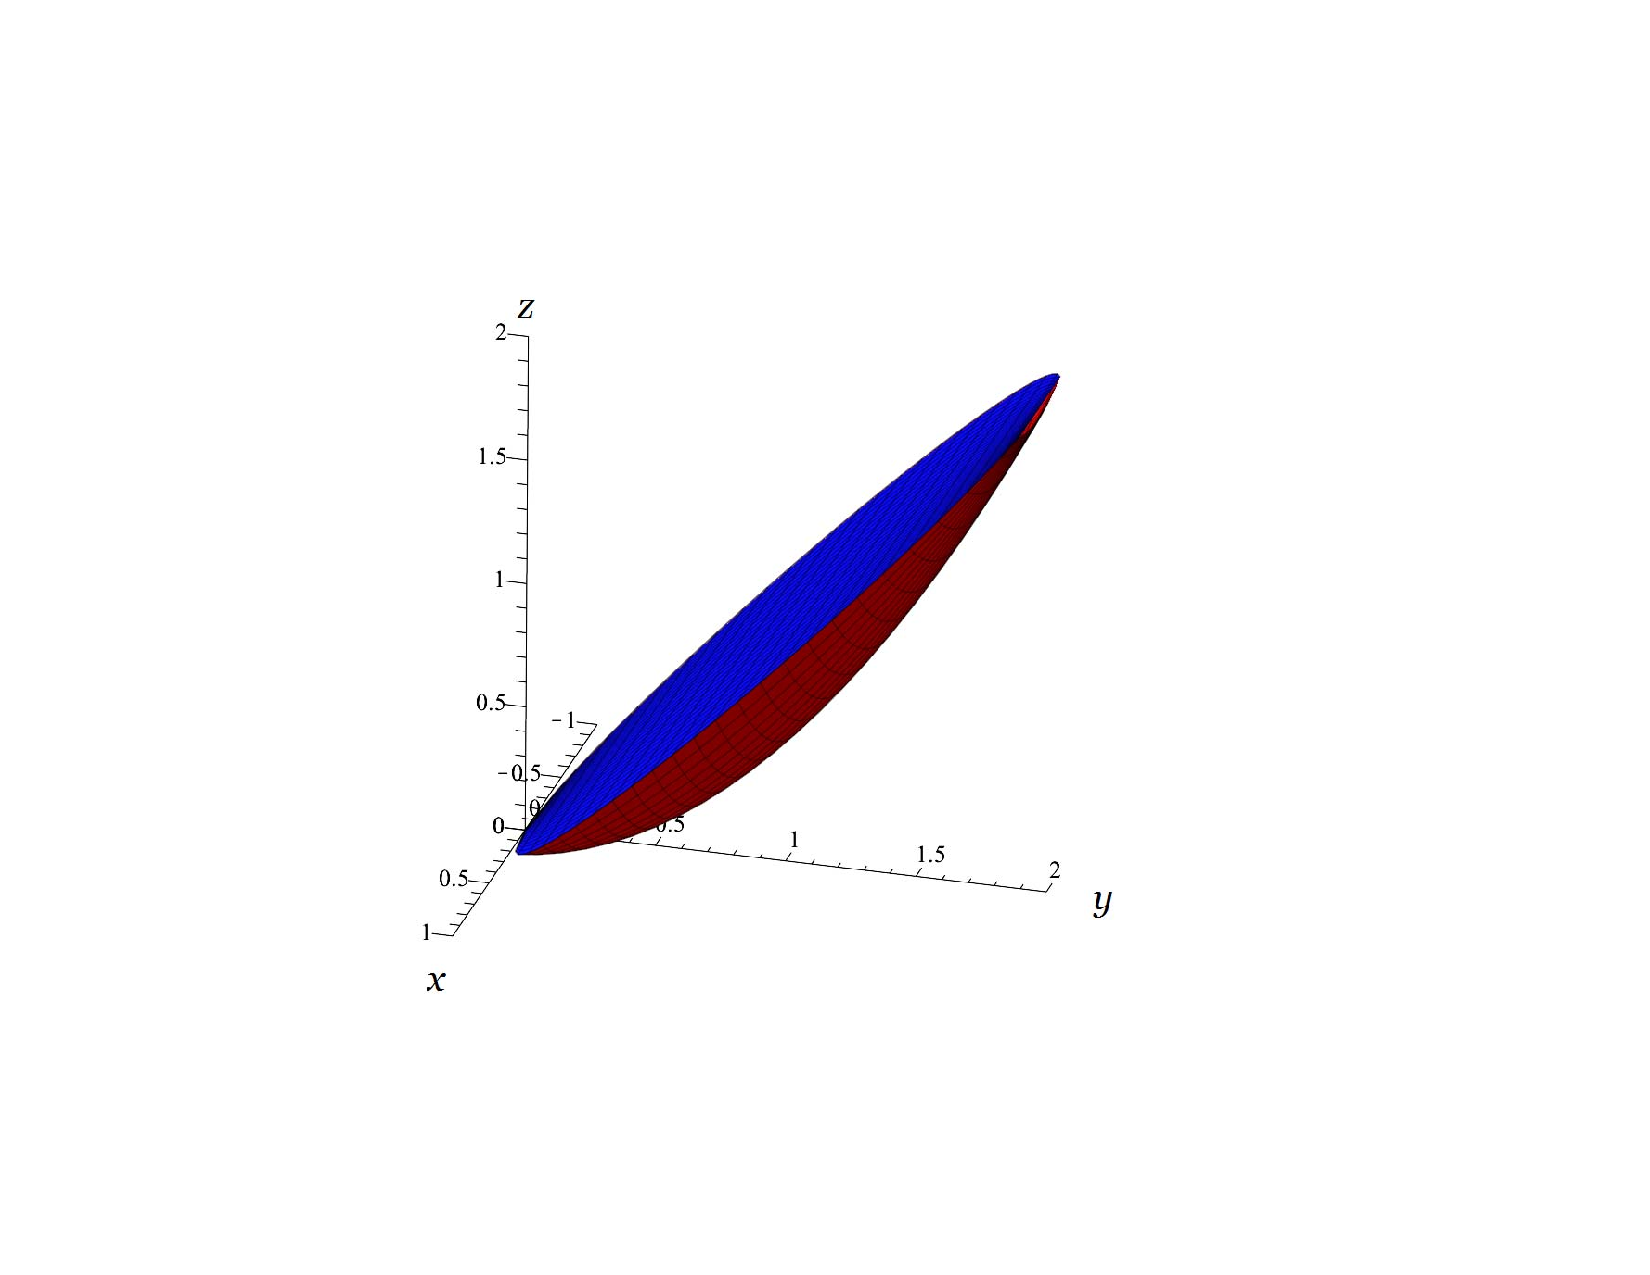
\includegraphics[scale=0.4]{slice.pdf}}} \fi

\item Match each equation to an appropriate graph from the table below.

\begin{enumerate}

\item $x^2-y+z^2=0$ 

\item $4x^2-9y^2+36z^2=-36$

\item $4x^2+4y^2+4z^2=36$ 

\item $x^2+z^2=16$

\item $x^2+z-y^2=0$

\item $4x^2-36y^2+9z^2=36$

\ifans{\fbox{\parbox{0.3\linewidth}{\begin{tabular}{c|c}
{\bf Equation} & {\bf Graph}\\
\hline
a& V\\
b& III\\
c& I\\
d& IV\\
e& II\\
f& VI
\end{tabular}}}}  \fi

\end{enumerate}

\begin{center}
\begin{tabular}{|lc|lc|}
\hline
(I) & & (IV)&\\
&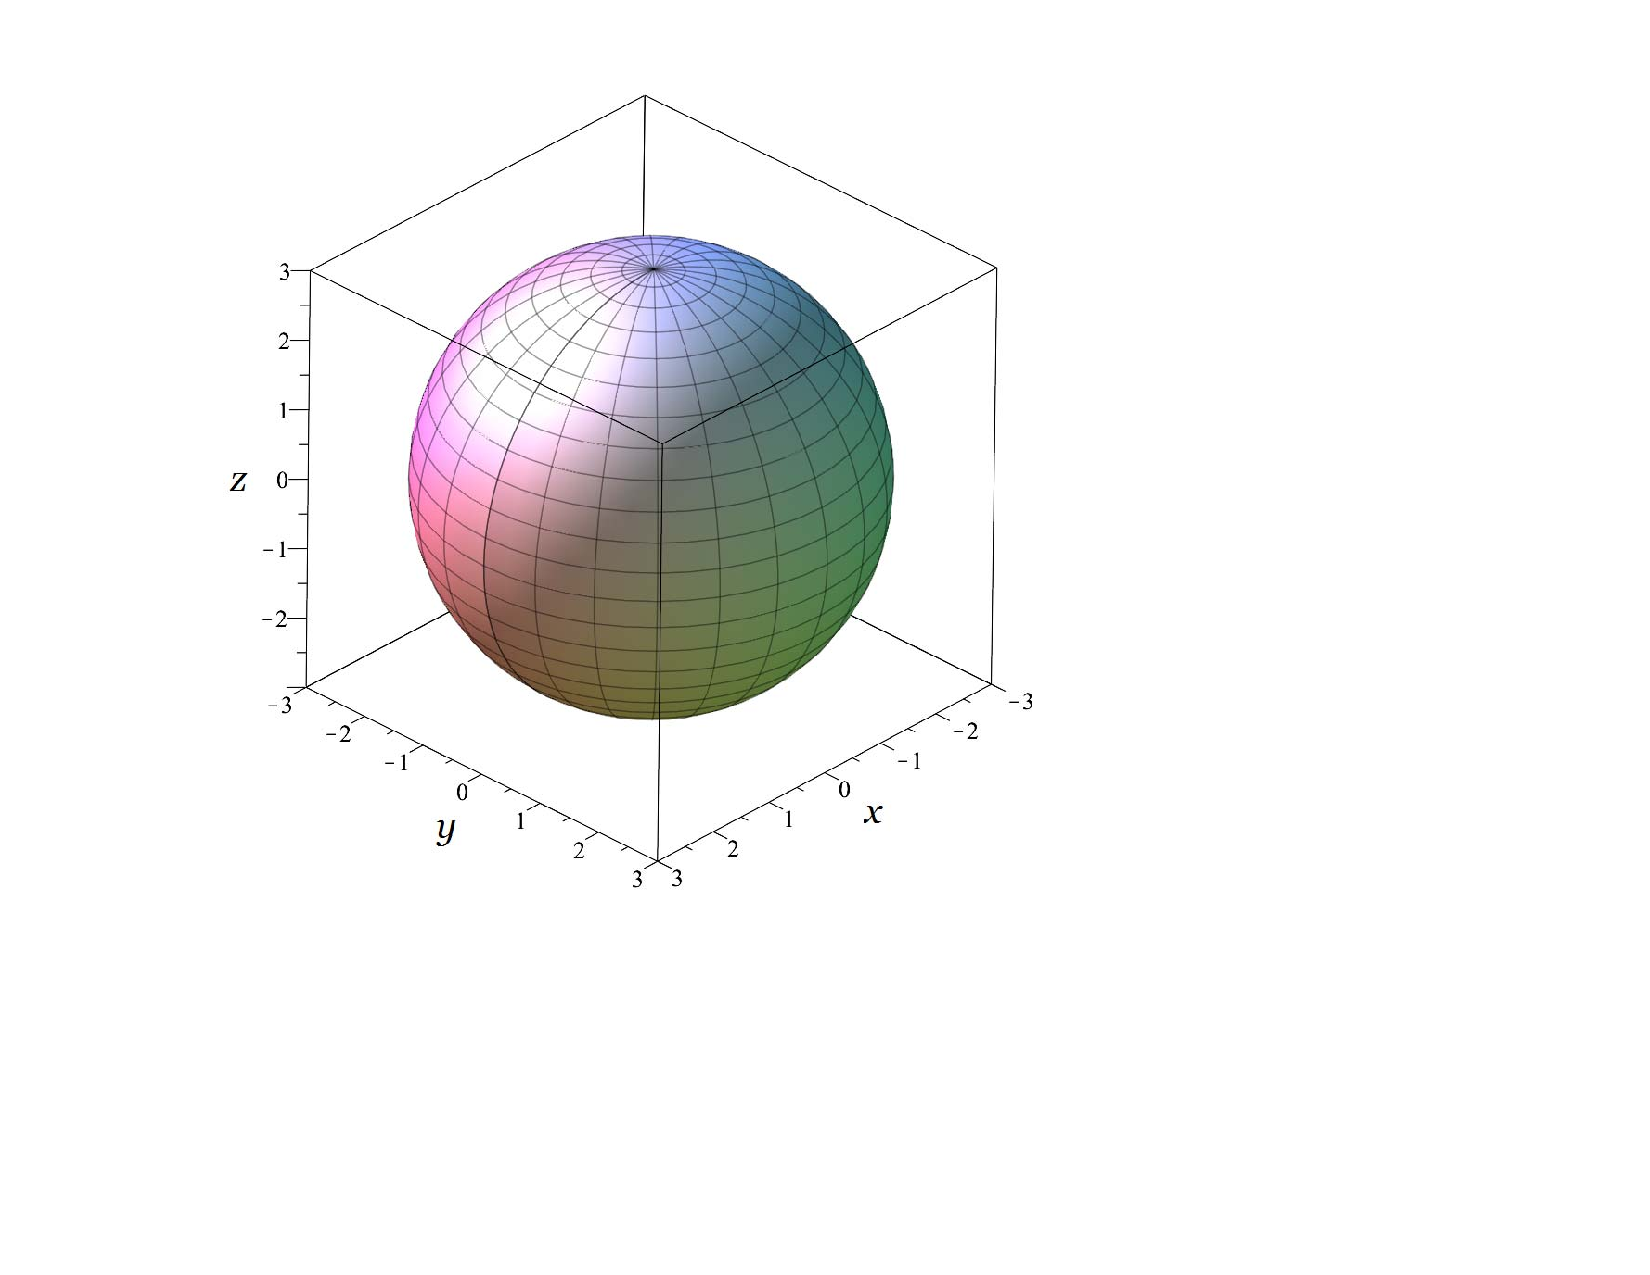
\includegraphics[scale=0.4]{matching3.pdf}&&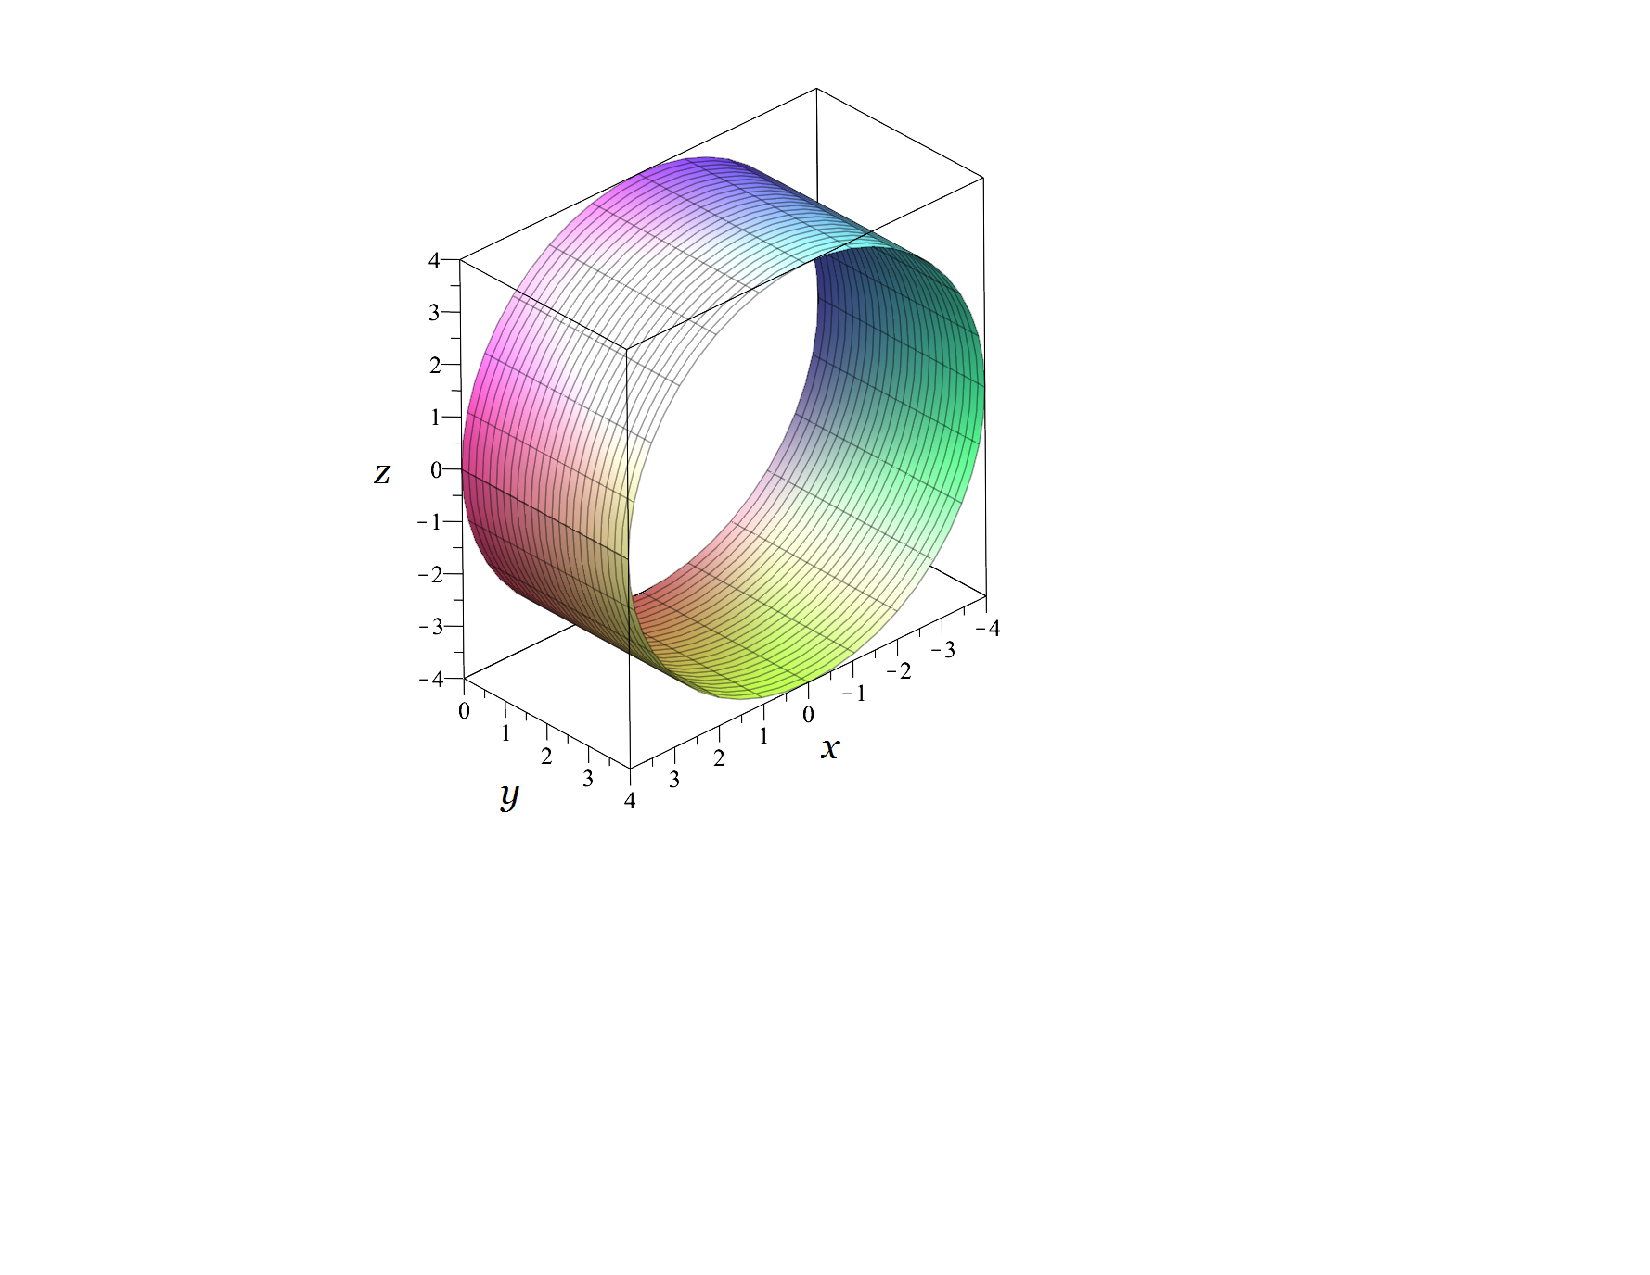
\includegraphics[scale=0.4]{matching4.pdf}\\
\hline
(II) & & (V)&\\
&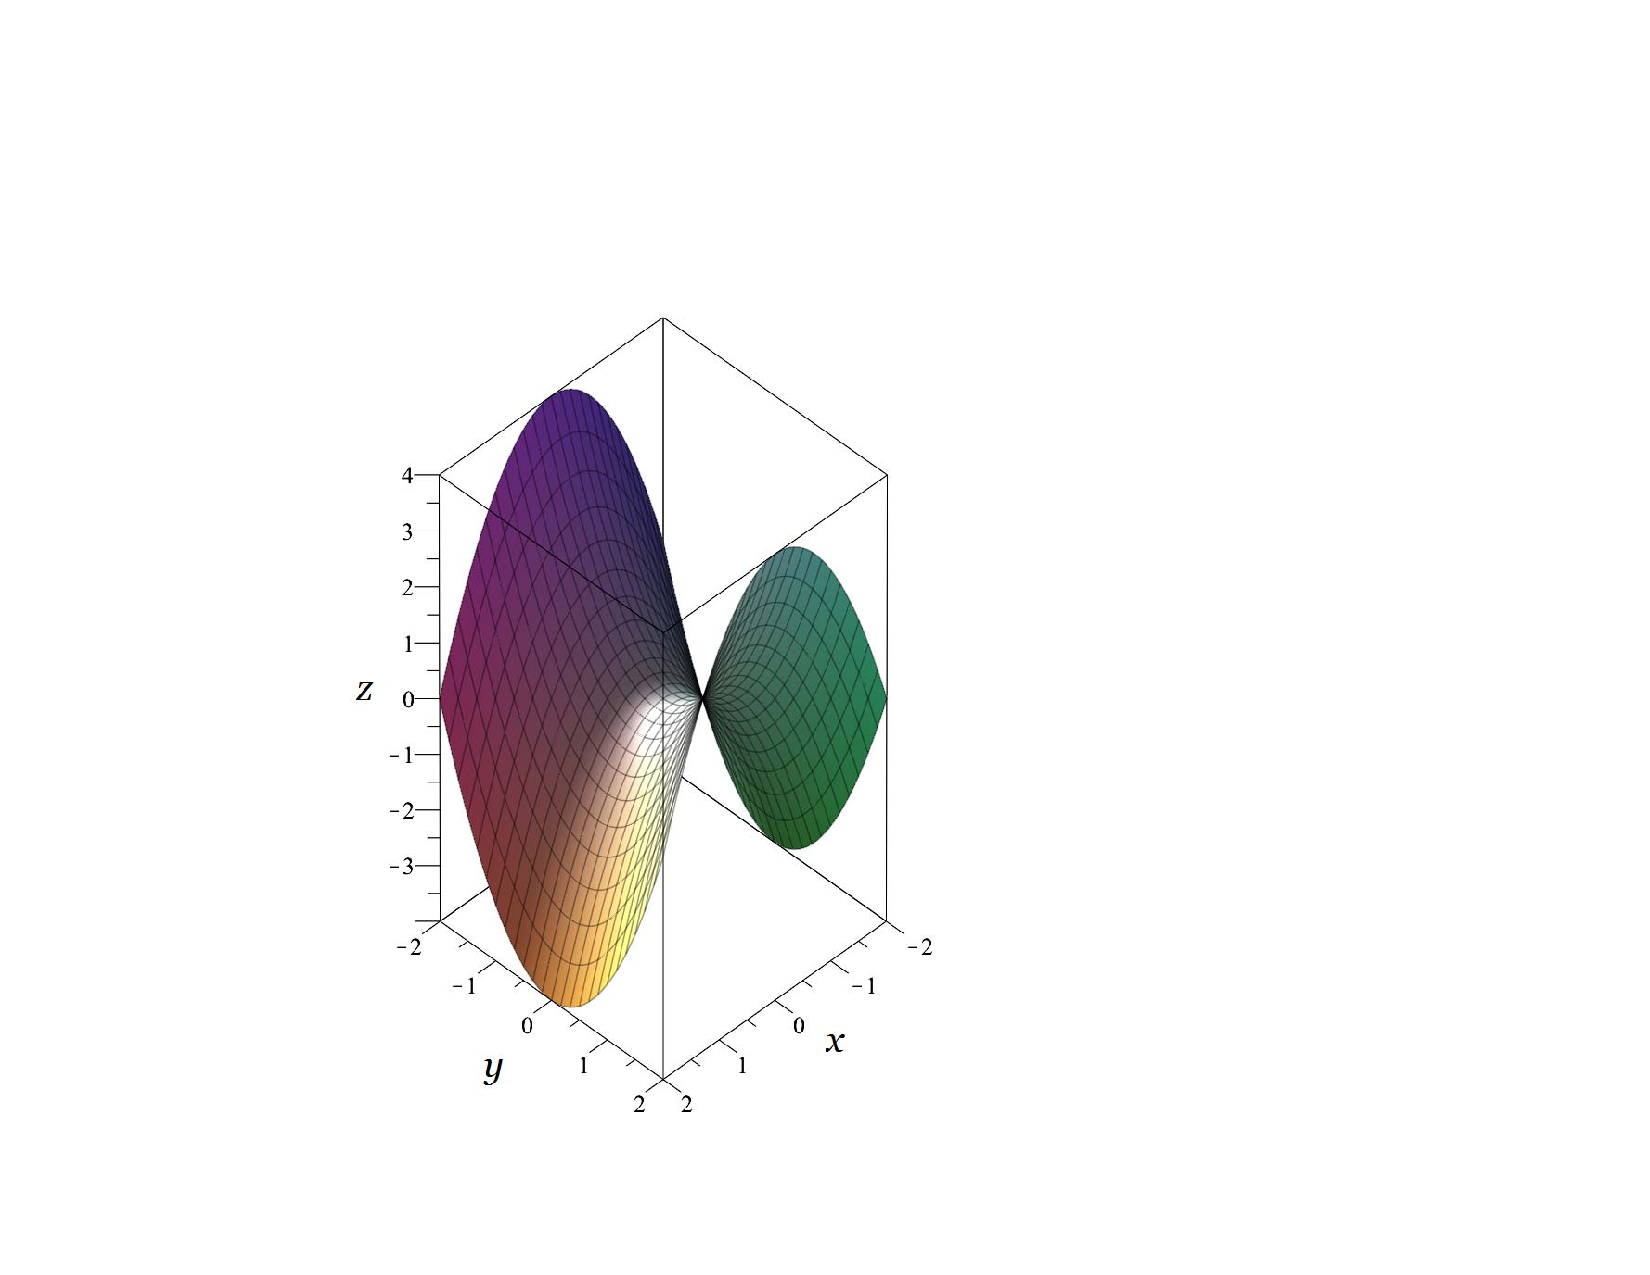
\includegraphics[scale=0.4]{matching5.pdf}&&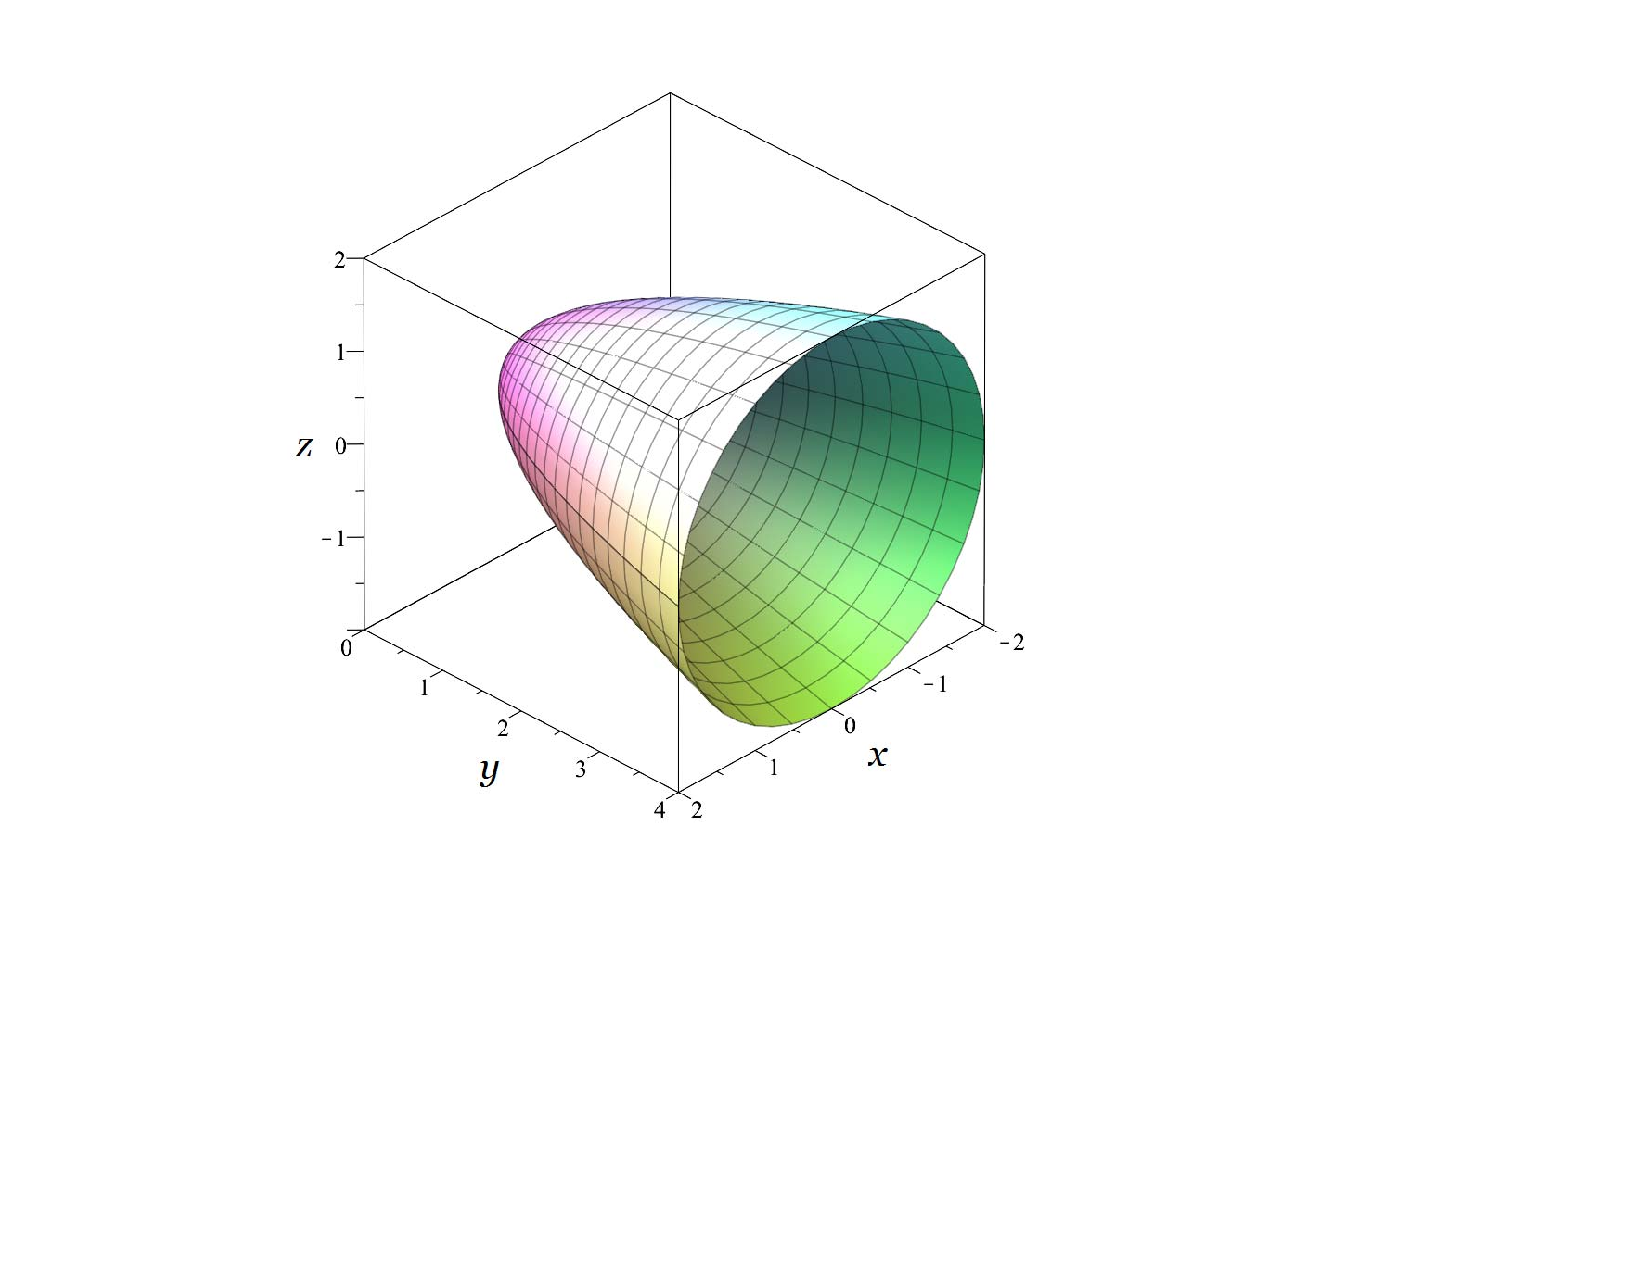
\includegraphics[scale=0.4]{matching1.pdf}\\
\hline
(III) & & (VI)&\\
&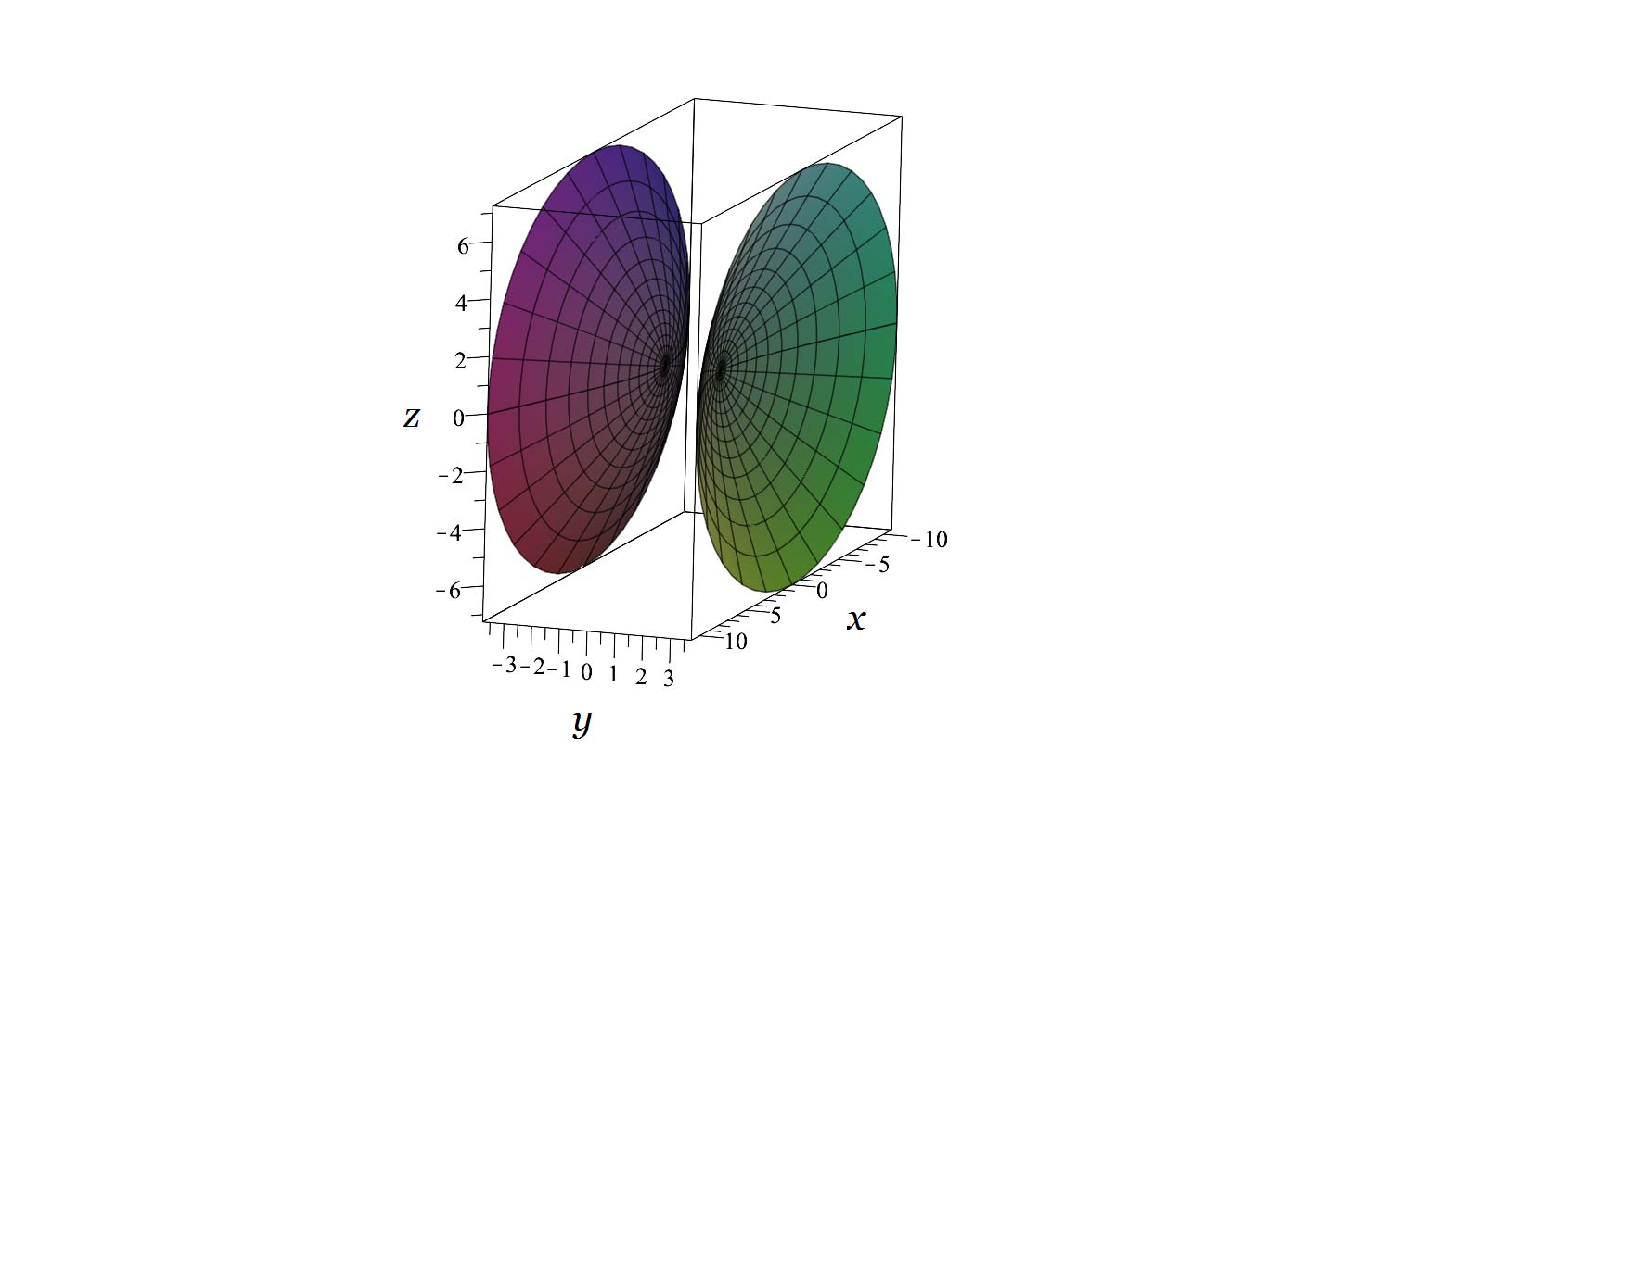
\includegraphics[scale=0.5]{matching2.pdf}&&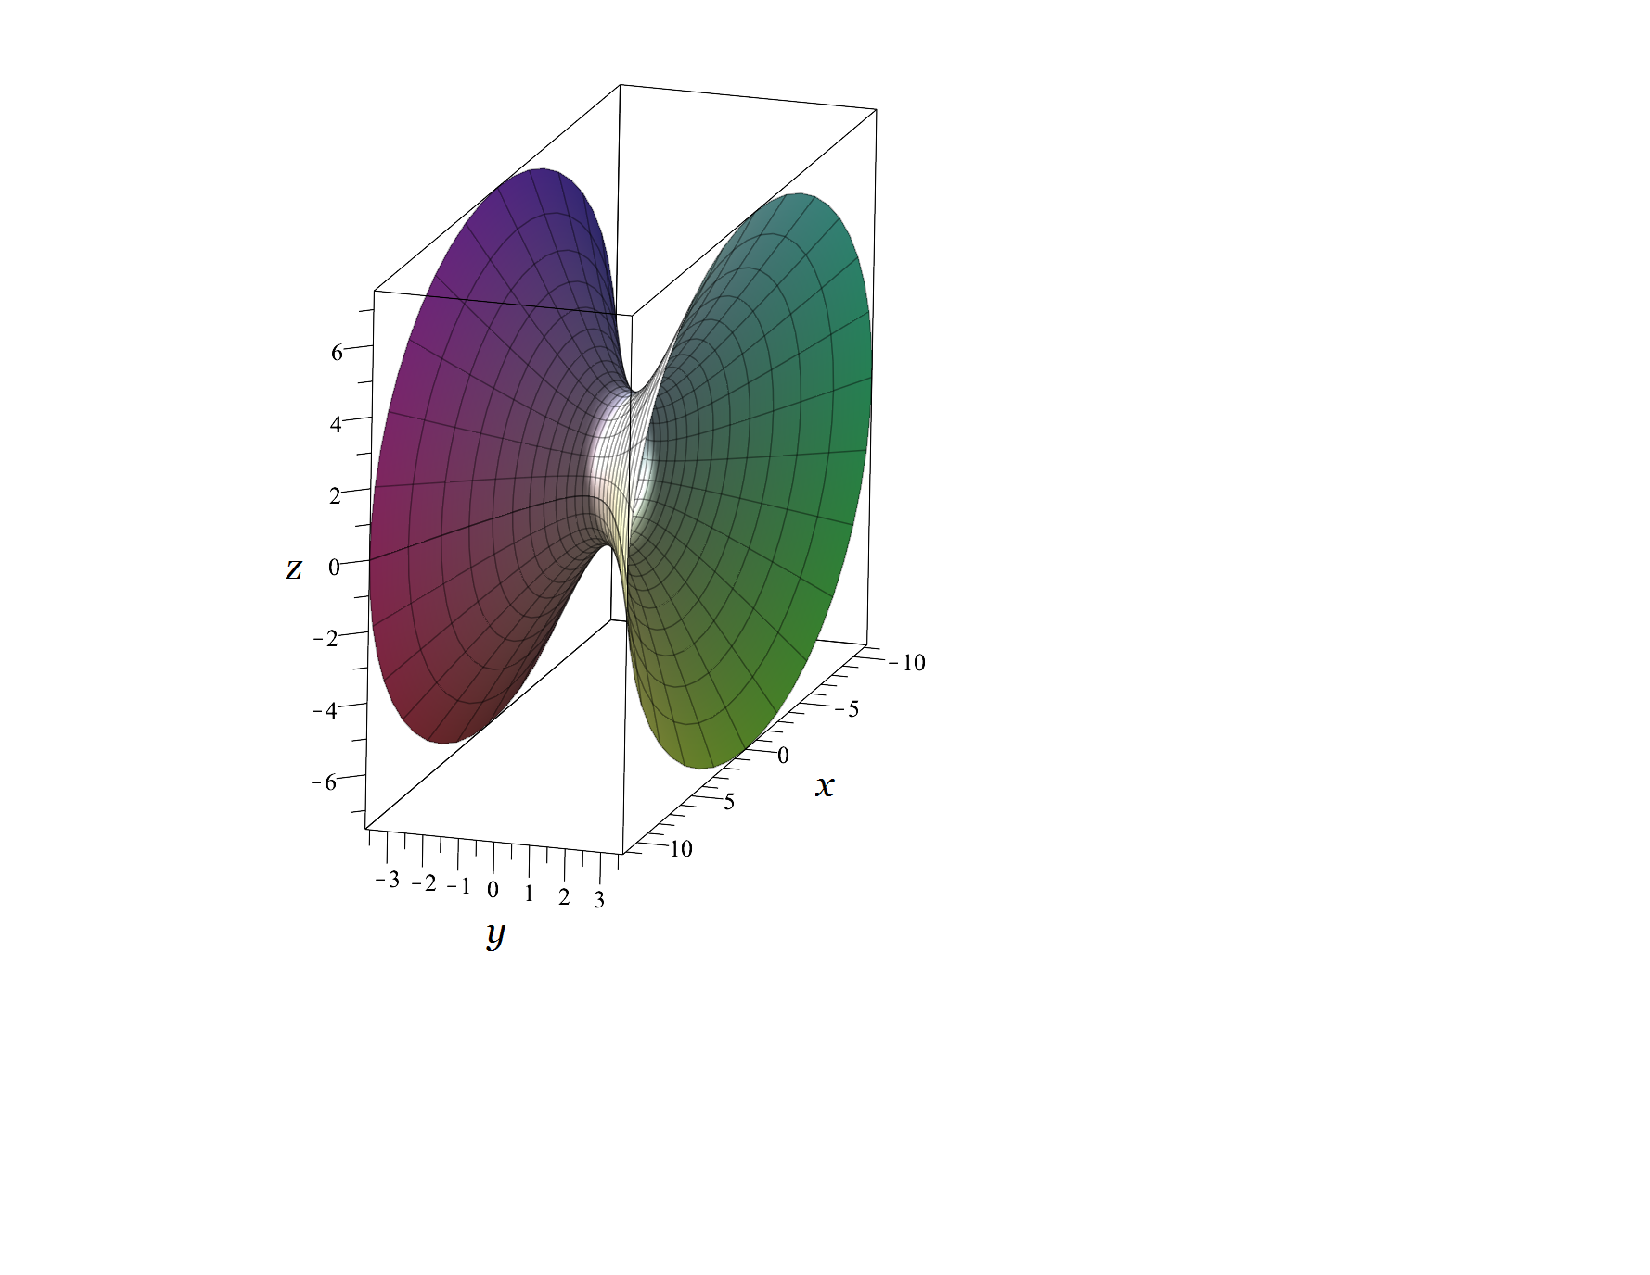
\includegraphics[scale=0.4]{matching6.pdf}\\
\hline
\end{tabular}
\end{center}

\end{enumerate}

\end{document}